\documentclass[a4paper, 12pt]{report}

\usepackage[tc]{titlepic}    % used to custom yourself title page
\usepackage{fontspec}
\usepackage{titlesec}
%\title{VLSI设计\\
%Norm指令的低功耗全定制设计}
%\author{\href{song_mh@yeah.net}{宋明辉$^\star \qquad$ 16063216}\\
%{$^\star$\textit{text}}}

\usepackage{geometry}
\geometry{left=3cm,right=3cm,top=1.8in}

\usepackage{makeidx}
\makeindex

\usepackage{xeCJK}
\setmainfont{Times New Roman}
\setCJKmainfont[BoldFont={SimHei}, ItalicFont={KaiTi} ]{SimSun}
\setCJKsansfont{SimHei}
\setCJKmonofont{SimSun}
\setCJKfamilyfont{myssfont}[BoldFont={SimHei}, ItalicFont={SimSun}]{SimSun}
\newcommand{\myss}{\CJKfamily{myssfont}}
\usepackage{indentfirst}

\usepackage{booktabs}
\usepackage{subfigure}
\usepackage{wrapfig}

\usepackage{multirow}     % for the use of multirow tables
\usepackage{amsmath}

\usepackage{fancyhdr}
\pagestyle{fancy}

\usepackage{graphicx}
\usepackage{xcolor}
\usepackage{caption}   % control how your captions will look like

\usepackage{booktabs}
%\usepackage{algorithmicx}
%\usepackage{algpseudocode}

\usepackage{clrscode3e}
\usepackage{listings}    % used to arrange the code

\bibliographystyle{plain}
\renewcommand\bibname{References}

\usepackage[colorlinks]{hyperref}

\renewcommand{\chaptermark}[1]{\markboth{#1}{}}
\renewcommand{\sectionmark}[1]{\markright{\thesection\ #1}}
\fancyhf{}
\fancyfoot[C]{\bfseries \thepage}
\fancyhead[LO]{\bfseries \rightmark}
\fancyhead[R]{\bfseries \leftmark}
\renewcommand{\headrulewidth}{0.3pt}
\renewcommand{\footrulewidth}{0pt}

% define some colors
\definecolor{title}{RGB}{180, 0, 0}
\definecolor{other}{RGB}{171, 0, 255}
\definecolor{name}{RGB}{171, 0, 255}
\definecolor{phd}{RGB}{0, 0, 240}

% Change the section font style
%\titleformat*{\section}{\Large \itshape}
%\titleformat*{\subsection}{\large \itshape}
%\titleformat*{\subsubsection}{\itshapte}

\begin{document}
% custom design myself title page
\begin{titlepage}
\begin{center}

{
\vfill
\large \bfseries VLSI设计 \\ [5pt]
\Large Norm指令的低功耗全定制设计
}\\
% -----------------------------------
\vspace{1.5cm}
{
\Large \textit{Triloo} 
}\\
% -----------------------------------
\vspace{7cm}
\textsc{{\large 国防科技大学 计算机学院}} \\ [5pt]
\vspace{2cm}
%\vfill
% -----------------------------------
{
\includegraphics[width=0.2\textwidth]{Nudt}} \\[5pt]
\vspace{0.5cm}
\today

\end{center}
\end{titlepage}
%\maketitle    % do not need \maketitle anymore
\tableofcontents
\date{}        % remove the default date information

% use new geometry setting, use \restoregeometry to use the default setting
\newgeometry{left=3cm,right=3cm,top=1in}
%\geometry{left=3cm,right=3cm,top=1in}

\chapter*{报告说明}
\addcontentsline{toc}{chapter}{报告说明}
本次实验主要完成tms320 DSP的NORM指令的全定制设计,设计流程为:电路图设计、功能验证、时序分析与电路优化、版图设计与验证等步骤,主要包括31位反向器、2路31位选择器、以及前导零检测电路等子模块。其中,前导零模块的设计参考''Low-power leading zero counting and anticipation''\cite{dimitrakopoulos2008low}一文,即通过逻辑优化,尽可能的降低需要用到的器件的数量来降低电路的功耗,具体内容参考第一章节中设计思路一节。最后,基于以上子模块,完成NORM指令的全定制设计,并通过DRC、LVS检查。

\chapter{功能与结构设计}
本章节将给出Norm命令的基本功能以及全定制实现的总体结构图等。
\section{指令功能}
\indent  首先Norm指令具有如下形式:
\begin{center}
\textbf{NORM} (.unit)  $\quad$ \textit{src2, dst}
\end{center}
%{\centering  } 
其过程涉及两个操作数,\textit{src2}为输入操作数,\textit{dst}为目的操作数,位宽均为32位。需要实现的功能如下:
\begin{quote}
The number of bits of the first nonredundant sign bit from the MSB of the src2
operand is placed in dst.
\end{quote}

\indent 该指令的功能即根据符号位的数值统计前导零或一的数量,若符号位为1,则统计符号位后前导一的位数,否则统计符号位后前导零的位数。例子如图\ref{fig1.1}所示:
\begin{figure}[!hbpt]
\centering
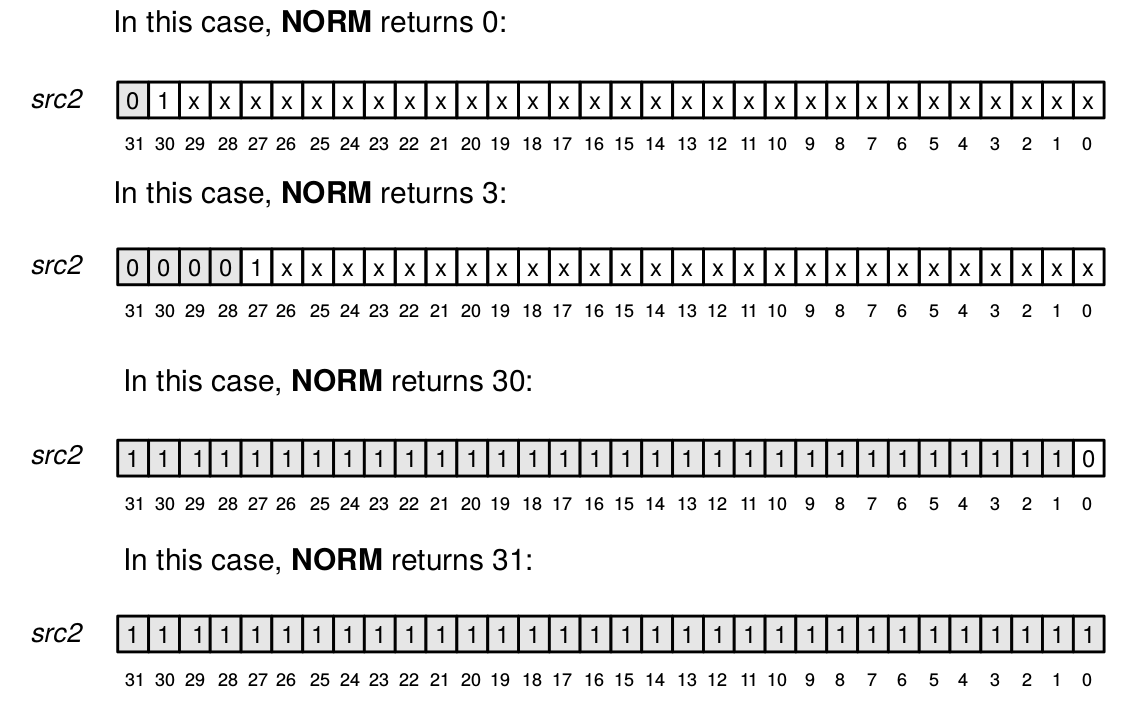
\includegraphics[width=0.8\textwidth]{chapter1/Norm_Example1}
\caption{NORM指令功能示例}
\label{fig1.1}
\end{figure}\\
并要求该指令需要在一个时钟周期以内完成运算。存在多种电路可以完成该指令的功能,但本次实验仅选择基于''前导零计数''的方式对其进行实现。
\section{设计思路及总体结构图}
本小节将给出NORM指令的设计思路,即各个子模块的原理,然后给出NORM指令的总体结构图。
\subsection{设计思路}
通过对上述指令的说明进行分析可以发现,该指令的功能为计算符号位后连续1或0的个数,连续零的个数可以通过前导零计算的模块进行,而前导1的个数可以通过先将输入操作数进行按位取反后再进行前导零的统计。
\subsubsection{前导零计算(LZC)模块}
通过以上讨论,可以明确前导零计数模块(LZC, Leading Zero Count Unit)的设计对NORM指令的实现至关重要。目前同样存在多种计算前导零的实现方法,文章\cite{dimitrakopoulos2008low}中给出了三种已有的计算方法,下面对其进行简单说明。在本章节的最后一部分中,给出该篇文章实现的低功耗改进方法,这也是本次实验采用的方案。
\begin{itemize}
\item \textbf{Encoder-Based LZC Unit}\\
第一种方法是基于两步编码过程的实现电路。首先检测Leading Digit(即前导零统计过程中的第一位不为零的位,前导1的统计过程中类似。),并将检测结果编码成One-Hot编码形式,如输入为00110100,则第一步的编码结果输入为00100000。为了得到One-Hot码,引入中间变量$S$,与One-Hot码不同的是,该中间变量在leading digit位之后的所有位都为1,例如同样输入00110100时,中间变量$S$为00111111。设$S$的第$i$位表示为$S_i, 0 \le i \le n-1 $,定义如下:
\begin{equation}\label{equ1.1}
S_i = A_{n-1} + A_{n-1} + \cdots + A_{i+1} + A_i
\end{equation}
其中$+$表示逻辑或运算。从公式\ref{equ1.1}可以看出$S_i$的含义为最高位与$i_th$位之间是否存在为1的位。在得到中间变量$S$后,通过将$S$的连续两位的数值来得到One-Hot码(用$L$表示):
\begin{equation}\label{equ1.2}
L_i = \overline{S}_{i + 1} \cdot S_i = \overline{S}_{i + 1} \cdot A_i \quad (0 \le i \le n-2)
\end{equation} 
其中$L_{n-1} = S_{n-1}$。得到One-Hot码$L$的电路被称为优先编码器(Priority Encoder)。

在本方法中用到的第二个编码器是将得到的One-Hot码转换为类似'' 8421''码的有权码。例如,对于输入为8位的数值的转换过程可以表示为:
\begin{equation}
\label{equ1.3}
\begin{gathered}
Z_2 = L_3 + L_2 + L_1 + L_0\\
Z_1 = L_5 + L_4 + L_1 + L_0 \\
Z_0 = L_6 + L_4 + L_2 + L_0
\end{gathered}
\end{equation}
经过上述两次编码后,即完成前导零统计的过程。

\item \textbf{Algorithm-Based LZC Unit} \\
已有的第二种计算前导零的电路被称为基于算法的统计。在该方法中,首先将输入$n$位数值分成$n/2$个连续两位构成的Groups.对于每一Group实行前导零计算。接下来,相邻的两个Group的计算结果被组合,且基于左Group的结果对两个结果进行选择。然后经过$\log_2n $次迭代后即可实现前导零检测的功能。这种方法可以通过模块化的方式进行全定制实现,同时也是目前已知的最快的基于静态CMOS的前导零实现方法。其示意图如图\ref{fig1.2}所示:
\begin{figure}[!hbtp]
\centering 
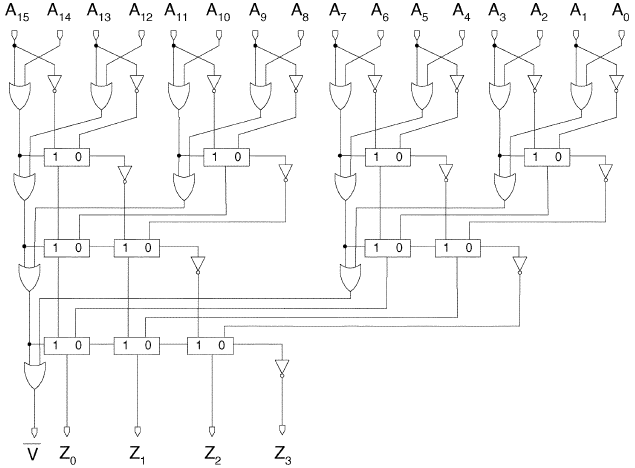
\includegraphics[width=0.9\textwidth]{chapter1/LZC_16bit}
\caption{Algorithm-based LZC的16-bit实现电路图}
\label{fig1.2}
\end{figure}
\item \textbf{Recursively-Based LZC Unit}\\
这种方法通过迭代的方式计算LZC结果(用$Z$表示)的第$i$位。下面以8-bit的LZC结算过程为例进行说明。首先对最高的4位进行$A_7A_6A_5A_4$检测,若此四位全为零,则说明输入的数值$A$中至少存在4个0,因此将$Z_2$置位,即得到$Z_2 = 1$,这意味着我们还需要对$A_3A_2A_1A_0$进行检测并统计。接下来则需要对$A_3,Z_2$以及$A_7,A_6$进行检测,并基于检测结果来决定$Z_1$的具体数值,并根据$Z_2$的数值来决定具体是根据$A_3,Z_2$还是$A_7,A_6$来确定$Z_1$的数值,然后重复上述过程,直至完成LZC统计。
\end{itemize}
\subsubsection{低功耗前导零计算模块原理}
在这一部分,将给出低功耗前导零计算模块的具体设计思路,即文章\cite{dimitrakopoulos2008low}中的''PROPOSED LZC ALGORITHM''一节。首先,将公式\ref{equ1.2}带入公式\ref{equ1.3}中可以得到如公式\ref{equ1.4}所示的结果:
\begin{equation}
\label{equ1.4}
\begin{gathered}
Z_2 = \overline{S}_4 \cdot S_3 + \overline{S}_3 \cdot S_3 + \overline{S}_2 \cdot S_1 + \overline{S}_1 \cdot S_0 \\
Z_2 = \overline{S}_6 \cdot S_5 + \overline{S}_5 \cdot S_4 + \overline{S}_2 \cdot S_1 + \overline{S}_1 \cdot S_0 \\
Z_2 = \overline{S}_7 \cdot S_6 + \overline{S}_5 \cdot S_4 + \overline{S}_3 \cdot S_2 + \overline{S}_1 \cdot S_0 
\end{gathered}
\end{equation}
通过对$S_i$的计算过程分析可以发现,$(S_i, S_j)\; with \; i > j$不可能取$(1, 0)$的结果,基于这一性质可以对$Z$的计算过程进行简化,最终可以得到如下结果:
\begin{equation}
\label{equ1.5}
\begin{gathered}
Z_2 = \overline{S}_4 \\
Z_2 = \overline{S}_6 \cdot S_4 + \overline{S}_2 \\
Z_2 = \overline{S}_7 \cdot S_6 + \overline{S}_5 \cdot S_4 + \overline{S}_3 \cdot S_2 + \overline{S}_1
\end{gathered}
\end{equation}
然后利用公式\ref{equ1.2}的关系将公式\ref{equ1.5}中的变量$S_i$替换为输入$A$,即得到公式所示的输入与输出的关系:
\begin{equation}
\label{equ1.6}
\begin{gathered}
Z_2 = A_7 + A_6 + A_5 + A_4 \\
Z_2 = A_7 + A_6 + \overline{A}_5 \cdot \overline{A}_4 \cdot (A_3 + A_2) \\
Z_2 = A_7 + \overline{A}_6 \cdot A_5 + \overline{A}_6 \cdot \overline{A}_4 \cdot A_3 + \overline{A}_6 \cdot \overline{A}_4 \cdot \overline{A}_2 \cdot A_1
\end{gathered}
\end{equation}
最后,文章\cite{dimitrakopoulos2008low}给出了统一的计算LZC结果每一位$Z_i$的公式:
\begin{multline}\label{equ1.7}
F(X_{n-1}, X_{n-2}, \dots , X_{1}, X_{0}) = X_{n-1} + \overline{X}_{n-2} \cdot X_{n-3} + \\
+ \overline{X}_{n-2} \cdot \overline{X}_{n-4} \cdot \overline{X}_{n-5} + \cdots + \overline{X}_{n-2} \cdot \overline{X}_{n-4} \cdot \overline{X}_{n-6} \cdots \overline{X}_2 \cdot X_1
\end{multline}
基于公式\ref{equ1.7}的8-bit LZC计算过程如图所示:
\begin{figure}[!hbtp]
\centering
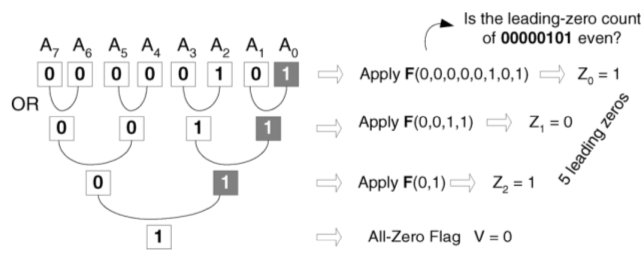
\includegraphics[width = 0.9\textwidth]{chapter1/LZC8bit}
\caption{8-bit输入LZC计算过程示意图}
\label{fig1.3}
\end{figure}
\subsubsection{低功耗16-bit LZC电路图}
基于公式\ref{equ1.7}的关系,可以得到16-bit输入时的LZC电路图,如图\ref{fig1.4a}所示,同时文章中还给出了一种功耗优化的改进电路,如图\ref{fig1.4b}所示。{\color{red} 可以看出,功耗优化后的电路图用到的器件数量更少,连线更加简单,且可以模块化实现,因此易于全定制设计,本次实验将采用图\ref{fig1.4b}的电路完成NORM指令的LZC子模块的设计。}
\begin{figure}[!hbtp]
\centering
\subfigure[16-bit LZC电路]{
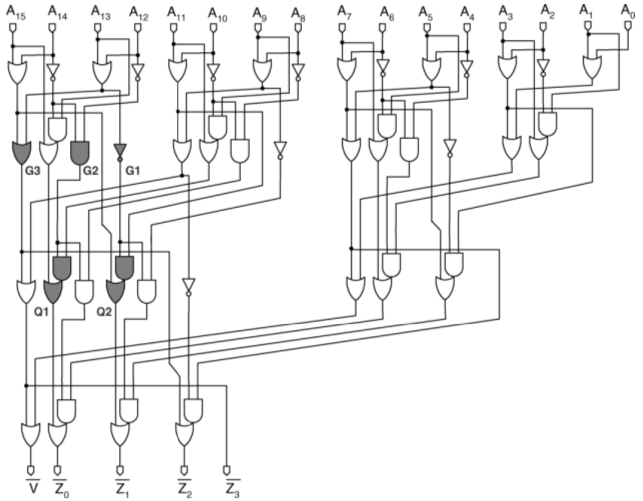
\includegraphics[width=0.45\textwidth]{chapter1/LZC16bit}
\label{fig1.4a}
}
\subfigure[功耗优化的16-bit LZC电路]{
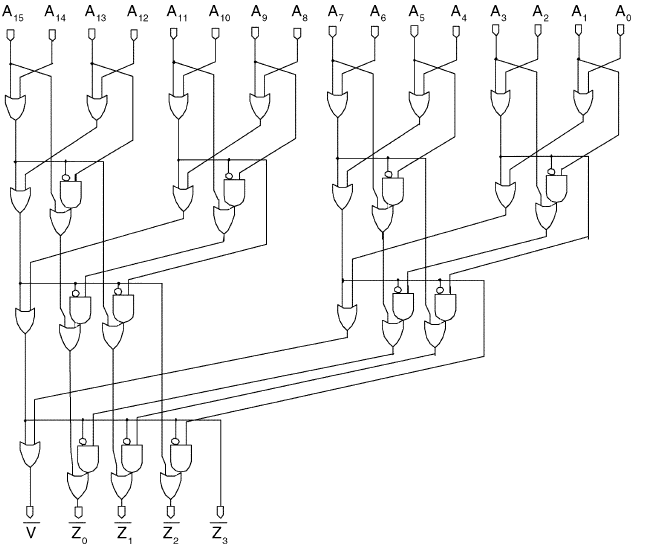
\includegraphics[width=0.45\textwidth]{chapter1/NewLZC16bit}
\label{fig1.4b}
}
\caption{16-bit的LZC电路及其功耗优化电路}
\label{fig1.4}
\end{figure}

关于低功耗LZC的设计更详细的信息可参考文章\cite{dimitrakopoulos2008low}。
\subsubsection{2路31位选择器的设计}
由于NORM指令除了需要检测前导零,还需要完成前导一的检测,因此,在设计过程中将输入的32位数据分成两路,一路将$0 \sim 31$位进行取反,另一路不做处理,并根据符号位是0还是1进行选择,即若符号位为1,则选择取反后的数据送入LZC电路,若符号位为0,则将不做处理的数据送入LZC电路。2路31位选择器的每一位基于图\ref{equ1.5}所示的1位选择器实现:
\begin{figure}[!hbtp]
\centering
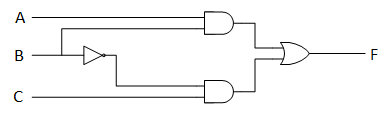
\includegraphics[width=0.9\textwidth]{chapter1/MUX2_1}
\caption{2路1位选择器单元}
\label{fig1.5}
\end{figure}\\
\noindent 其中,若$B$为0,则F为C端输入的数据,若$B$为1,则F为A端输入的数据。
\subsection{总体结构图}
基于以上讨论,可以得到NORM指令的总体结构图,如图\ref{equ1.6}所示。
\begin{figure}[!hbtp]
\centering
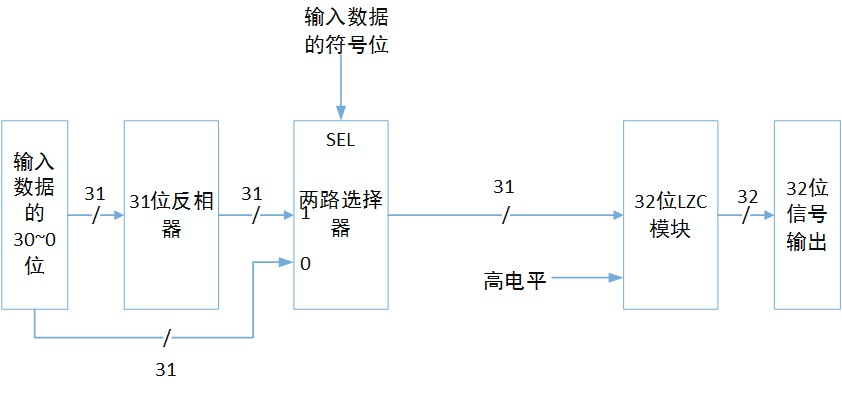
\includegraphics[width=0.9\textwidth]{chapter1/NORM}
\caption{NORM指令结构框图}
\label{fig1.6}
\end{figure}
\section{算法流程}
本小节将结合图\ref{equ1.6}对NORM指令的实现过程进行详细说明。

首先,输入数据的位宽为32位,由于NORM指令不仅需要计算符号位后连续0的个数,而且还要计算符号位后连续1的个数,因此为了实现电路复用,,选择将输入数据的$30 \sim 0$位数据分成两路,一路按位取反,一路不做任何处理,然后将31位反向器的结果与原始数据送入两路31位选择器,选择信号为输入数据的符号位,其工作原理为:若符号位为1则选择反向器的结果,否则选择原始数据。两路选择器的结果接下来被送往32位LZC模块,该模块实现前导零计算的功能。由于LZC是32位而输入数据是31位,因此还需要额外的一位数据输入到32位LZC中,且输入的数据不能影响NORM指令的正确性,因此在这里LZC的最低位的输入被设置为恒1。最后,将32位LZC的结果输出,此即为NORM指令的结果。


\chapter{电路图设计}
本章节将给出NORM指令的几个主要子模块的电路图设计,包括基本的与门、或门、反向器、多位选择器、LZC模块等。

图\ref{fig2.1}所示为主要单元的电路图设计。
\begin{figure}[!hbtp]
\centering
\subfigure[基本单元或非门]{
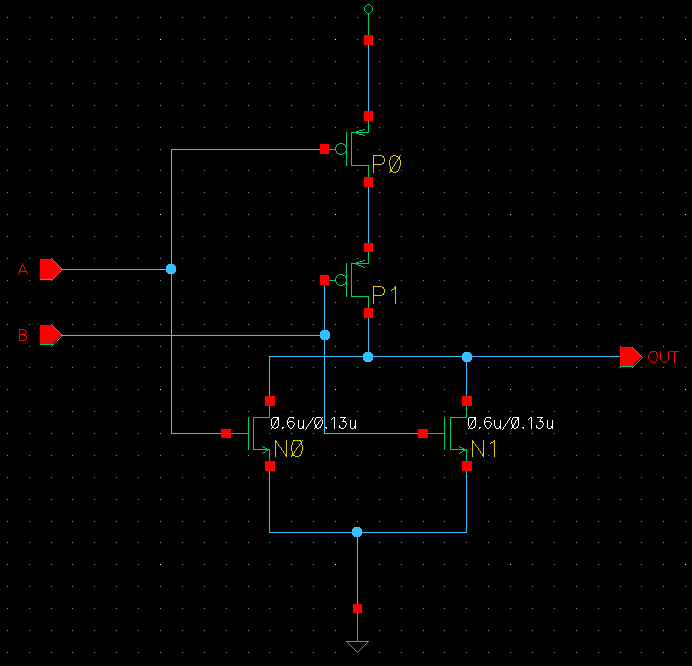
\includegraphics[width=0.4\textwidth]{chapter2/NOR}
\label{fig2.1a}
}

\subfigure[31位反向器]{
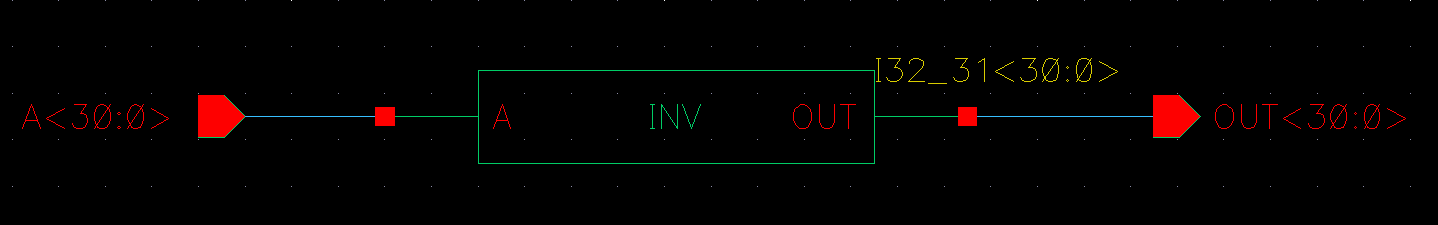
\includegraphics[width=0.4\textwidth]{chapter2/INV31}
\label{fig2.1b}
}

\subfigure[与或模块]{
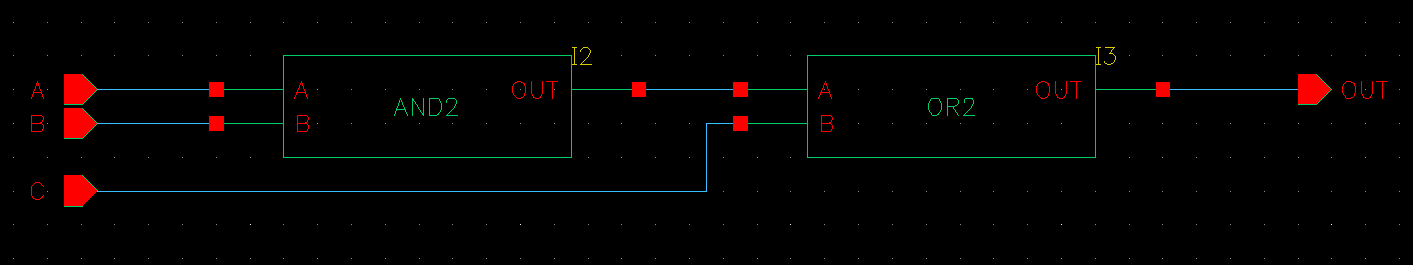
\includegraphics[width=0.4\textwidth]{chapter2/IAO}
\label{fig2.1c}
}

\subfigure[两路选择器]{
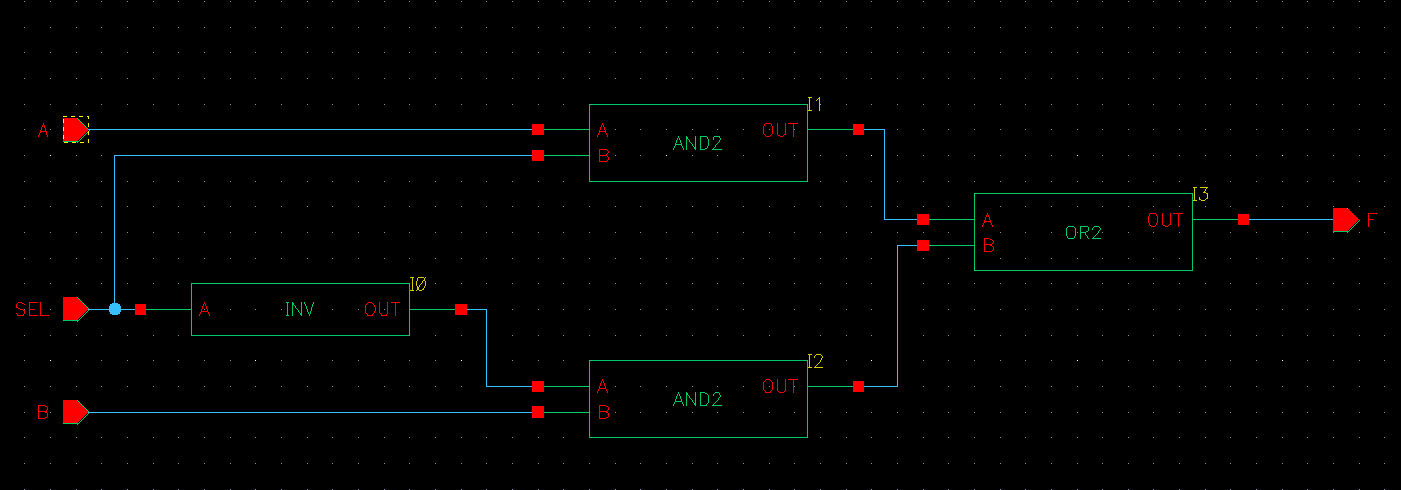
\includegraphics[width=0.4\textwidth]{chapter2/MUX2_1}
\label{fig2.1d}
}
\caption{主要基本单元的电路图设计}
\label{fig2.1}
\end{figure}\\
图\ref{fig2.2}为LZC模块的电路图设计,包括4-bit、16-bit、32-bit等不同层次。
\begin{figure}[!hbtp]
\centering
\subfigure[4-bit LZC模块]{
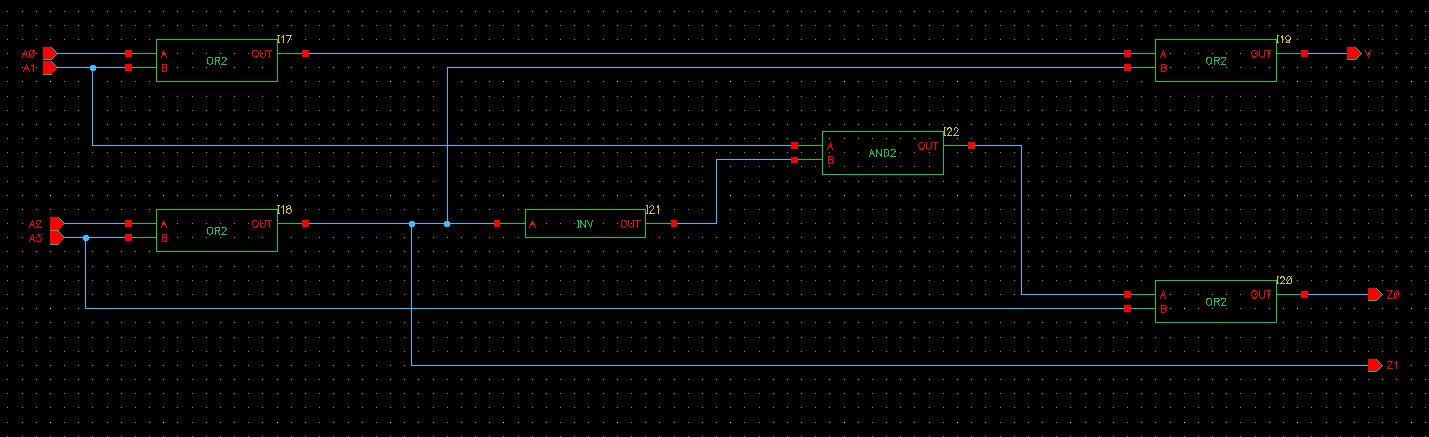
\includegraphics[width=0.6\textwidth]{chapter2/LZD4}
\label{fig2.2a}
}

\subfigure[16-bit LZC模块]{
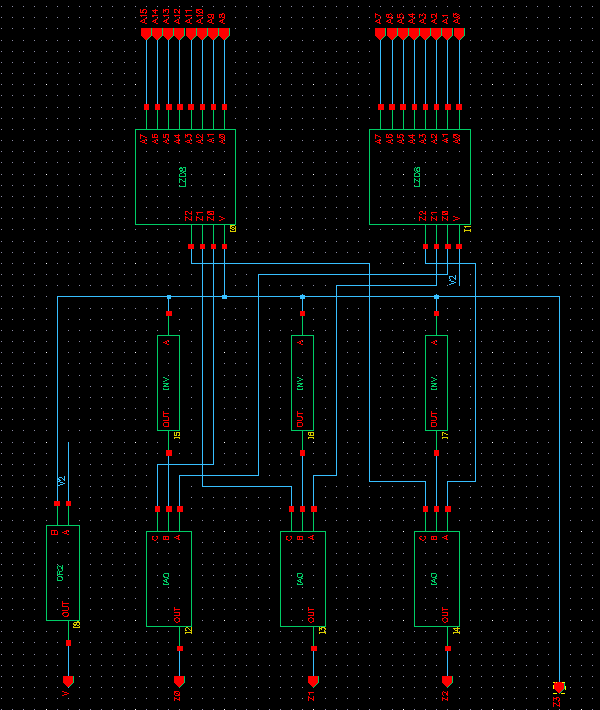
\includegraphics[width=0.5\textwidth]{chapter2/LZD16}
\label{fig2.2b}
}

\subfigure[32-bit LZC模块]{
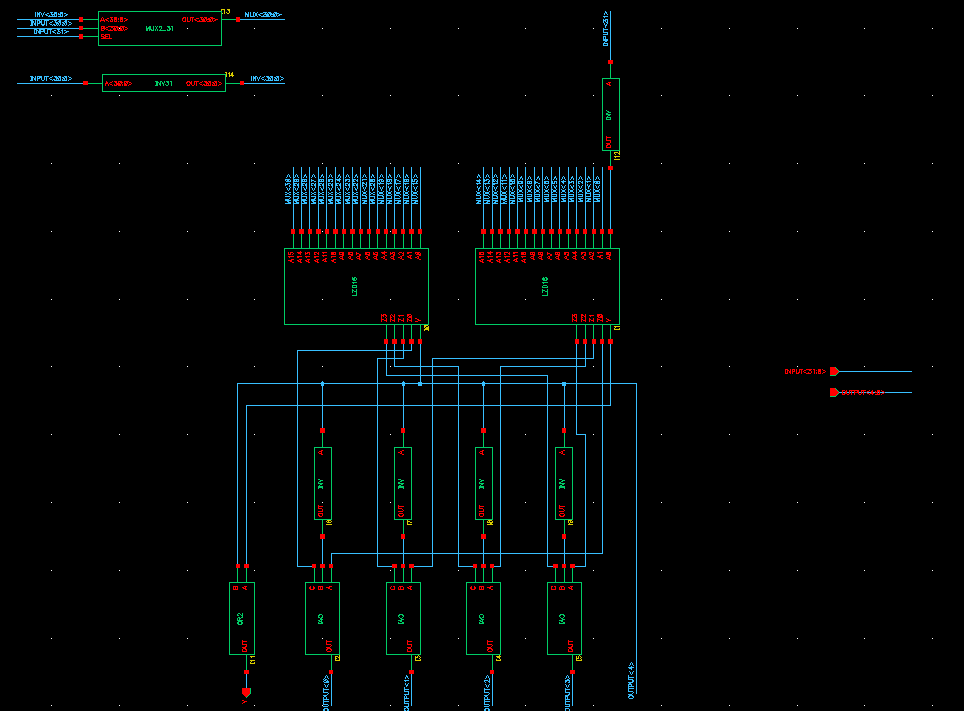
\includegraphics[width=0.65\textwidth]{chapter2/LZDF}
\label{fig2.2c}
}
\caption{主要基本单元的电路图设计}
\label{fig2.2}
\end{figure}\\
从图\ref{fig2.2}可以看出,32位LZC模块可由两个16-bit LZC子模块构成,此外还包括一个两路31位选择器,选择信号为输入操作数的符号位。需要注意的是,图\ref{fig2.2c}所示的模块的输出为6为,其中包括5位的LZC计算结果,还有1位信号$V$用于支持更宽的操作数。图\ref{fig2.3}为基于32位LZC模块以及NORM指令的功能要求实现的最终的电路图。此时,输出信号$V$被接地,且LZC计算结果被扩展为32位,高位($Lzc<31:5>$)通过27个反向器置零。
\begin{figure}[!hbtp]
\centering
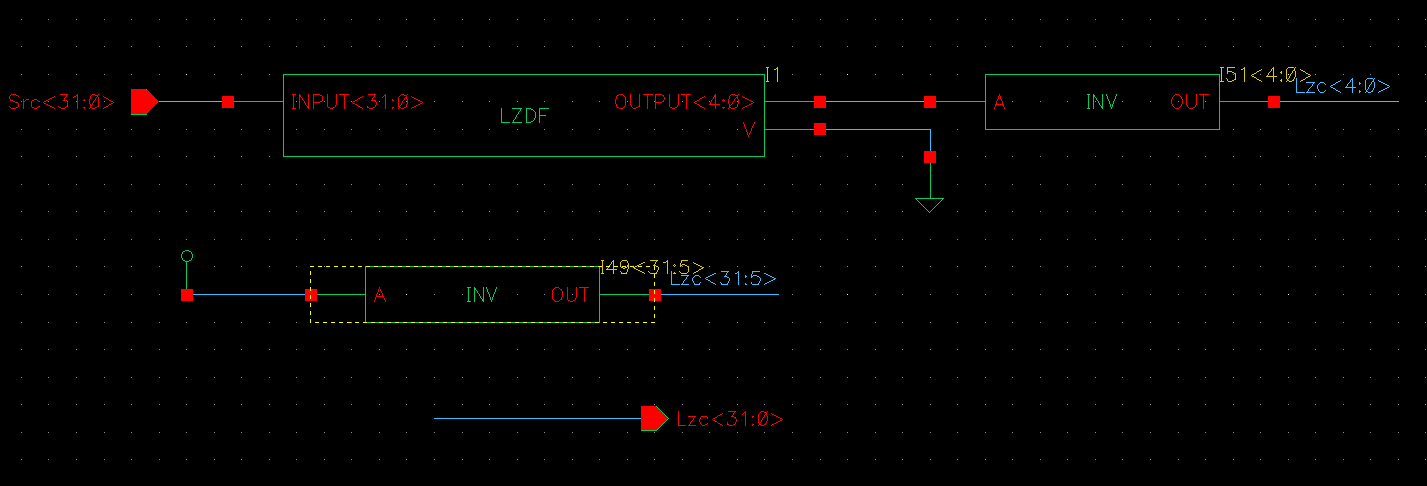
\includegraphics[width=0.9\textwidth]{chapter2/NORM}
\caption{NORM指令的实现电路}
\label{fig2.3}
\end{figure}

电路图中所有单元用到的NMOS、MPOS器件的长度均设为0.13um,NMOS的宽度设为0.6um,PMOS的宽度设为0.8um。



\chapter{功能验证}
本章节主要基于上一章的电路图设计进行功能验证,用到的主要工具软件为NC。
\section{NC简介}
NC-Verilog是Candence公司的Verilog数字逻辑模拟器,具有运行快、精度高、调试功能强大、使用灵活等优点,是业界公认的黄金模拟器。NC-Verilog的运行分为两个步骤,首先是编译,检查语法错误等,然后模拟执行。NC-Verilog使用NCC技术,提高了模拟的性能减少了内存的使用。采用INCA架构,具备了支持多种HDL语言、多设计层次、数模混合设计的能力。

运行流程包括:建立列表文件,列表文件包含激励信号;建立配置文件,以一个脚本的形式对NC进行配置,包括启动GUI界面、开启覆盖率统计、访问权限等设置;运行NC-Verilog,以上一步的配置启动NC;波形查看与调试,可以通过“shm\_open”和“shm\_probe”两个命令来保存波形,并且可以查看信号的波形以及逻辑结构图等,这一步主要通过查看波形以确定模块的正确性;查看覆盖率,这一步同样需要一个TCL脚本文件进行配置,并借助ICCR软件进行分析;导出VCD文件,可以通过tcl脚本或NC软件或“dumpfile”“dumpvars”来完成。以上就是功能验证部分的工作流程。 
\section{NC验证结果}
由于存在多个模块需要验证,为方便操作,在完成“或”模块的功能验证后,借助如下所示脚本来准备下一模块功能验证所需的文件以及部分内容等。

\lstinputlisting[language=sh,basicstyle=\footnotesize\ttfamily,caption={准备NC所需的文件脚本},label=list3.1]{chapter2/prefile.sh}
其中\verb|head -n 5 ./OR2/OR2_tb.v > $1/$1_tb.v|为准备各个子模块公用的Testbench信息,共5行,具体内容如下:
{
\footnotesize
\begin{verbatim}
`timescale 10ns/1ns
module cds_globals;
supply1 VDD_;
supply0 GND_;
endmodule
\end{verbatim}
}
\noindent Testbench剩下的内容即为根据具体模块的实例化以及激励的产生等。

图\ref{fig3.1}所示为基本单元的功能验证波形。
\begin{figure}[!hbtp]
\centering
\subfigure[二输入与的验证结果]{
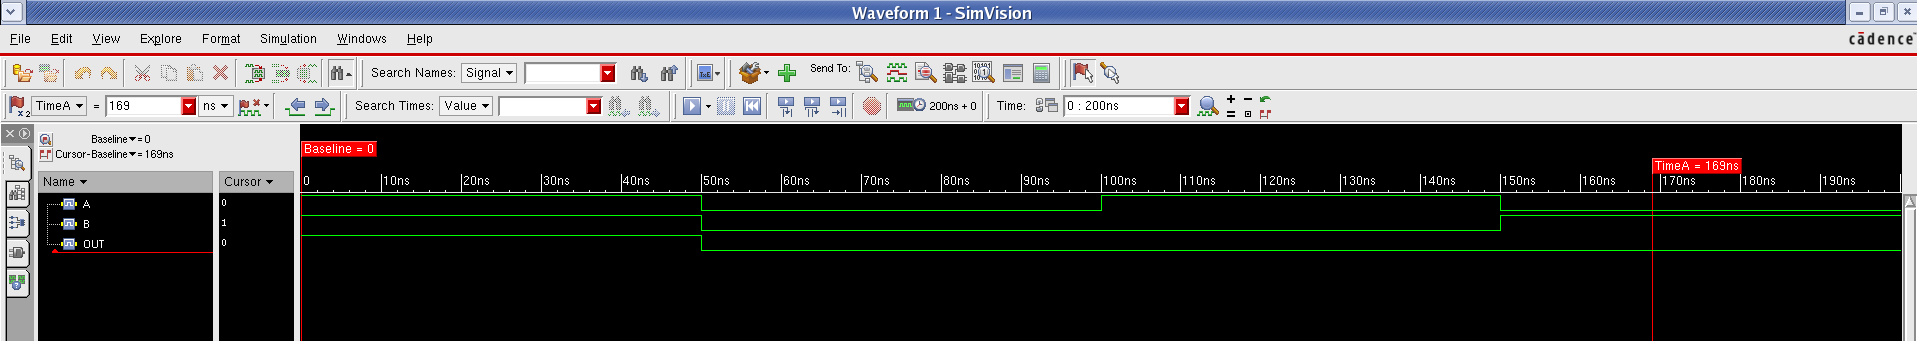
\includegraphics[width=0.9\textwidth]{chapter3/AND2_nc}
\label{fig3.1a}
}
\subfigure[三输入与或的验证结果]{
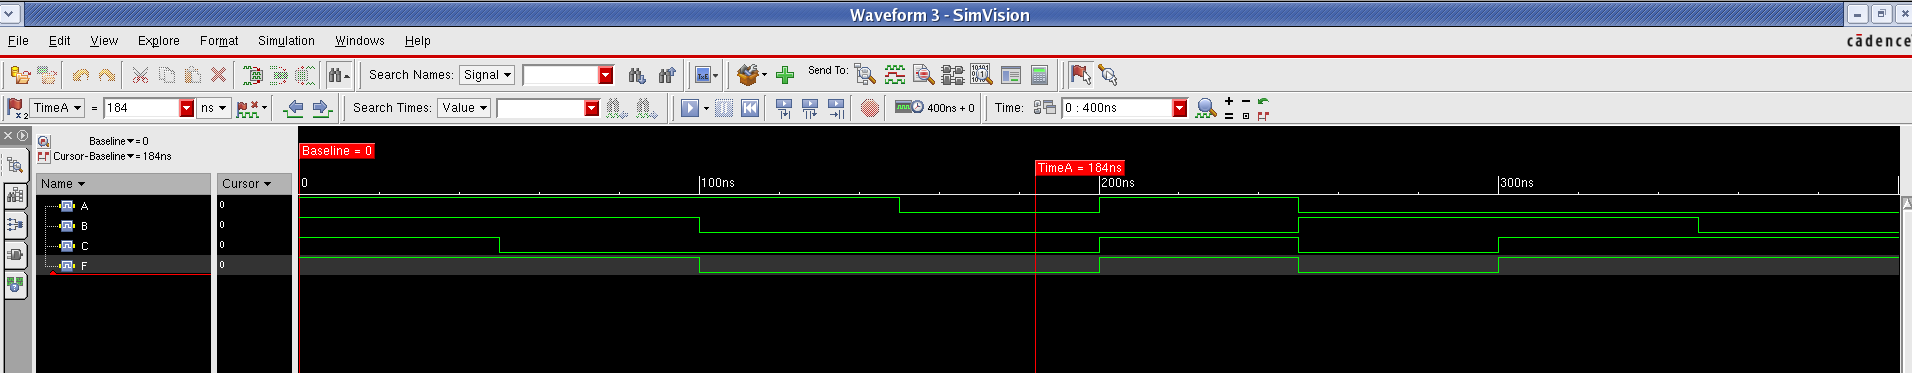
\includegraphics[width=0.9\textwidth]{chapter3/IAO_nc}
\label{fig3.1b}
}
\subfigure[两路31位选择器]{
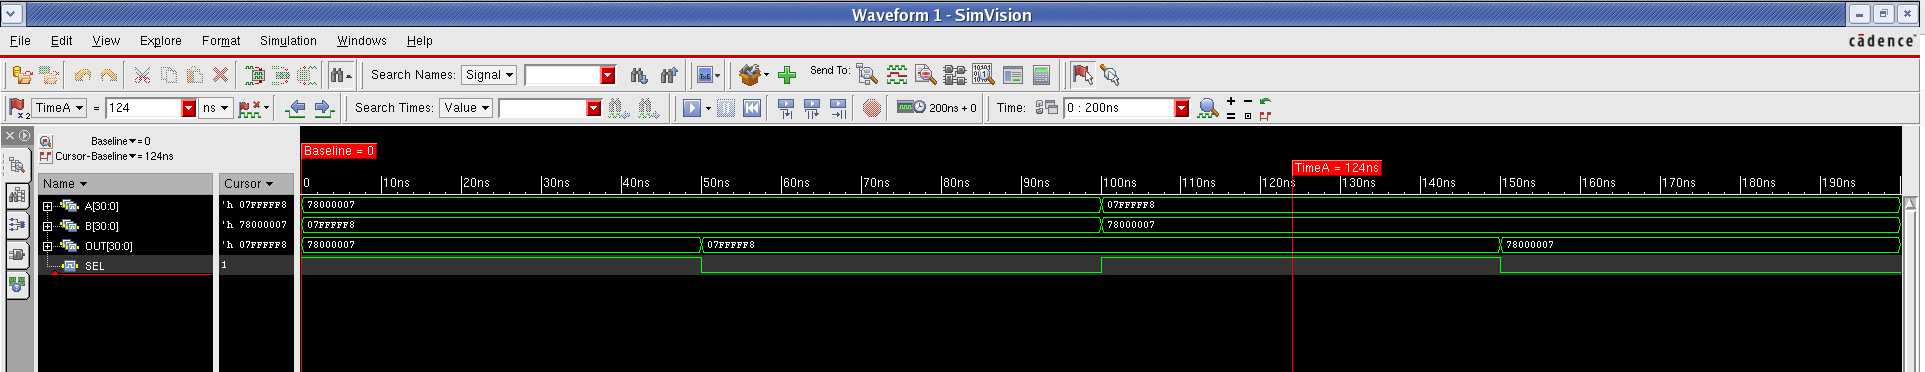
\includegraphics[width=0.9\textwidth]{chapter3/MUX2_31_nc}
\label{fig3.1c}
}
\caption{基本单元的NC验证结果}
\label{fig3.1}
\end{figure}\\
\indent 图\ref{fig3.2}所示为各级LZC模块的功能验证波形。
\begin{figure}[!hbtp]
\centering
\subfigure[4-bit LZC验证结果]{
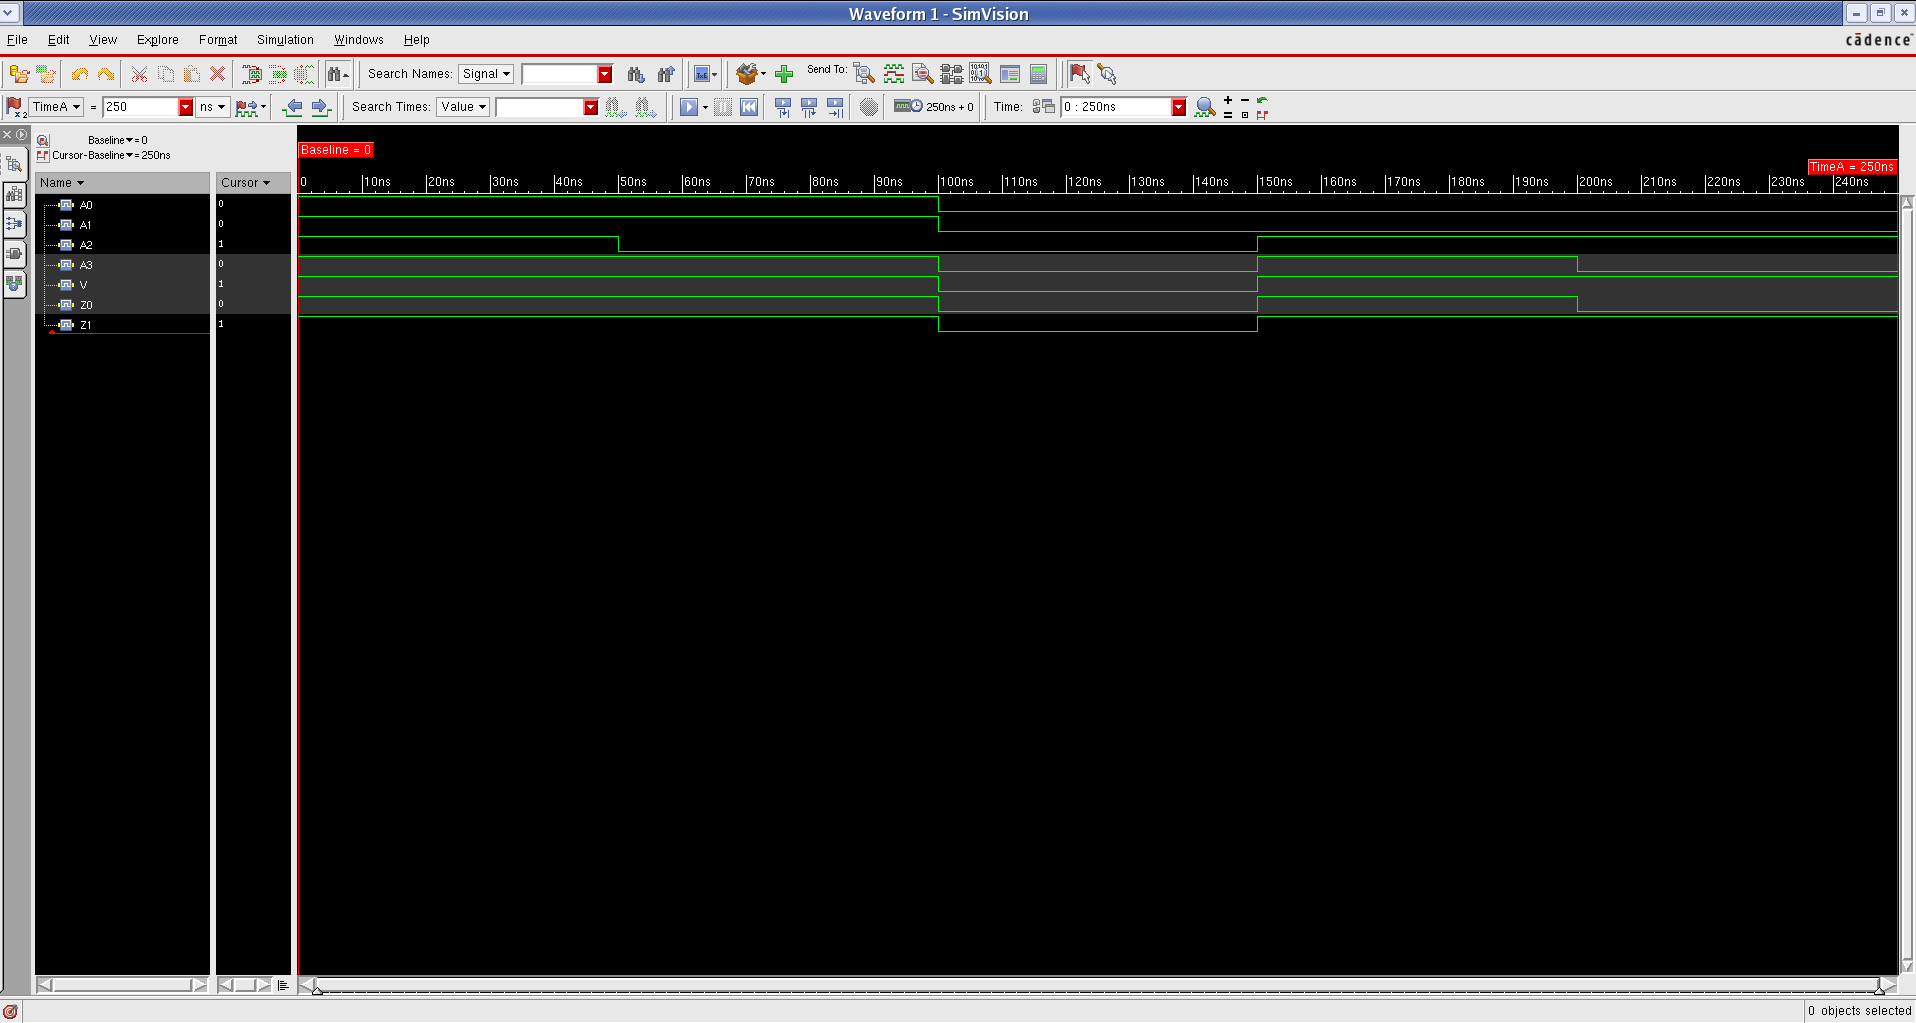
\includegraphics[width=0.9\textwidth]{chapter3/LZD4_nc}
\label{fig3.2a}
}
\subfigure[16-bit LZC验证结果]{
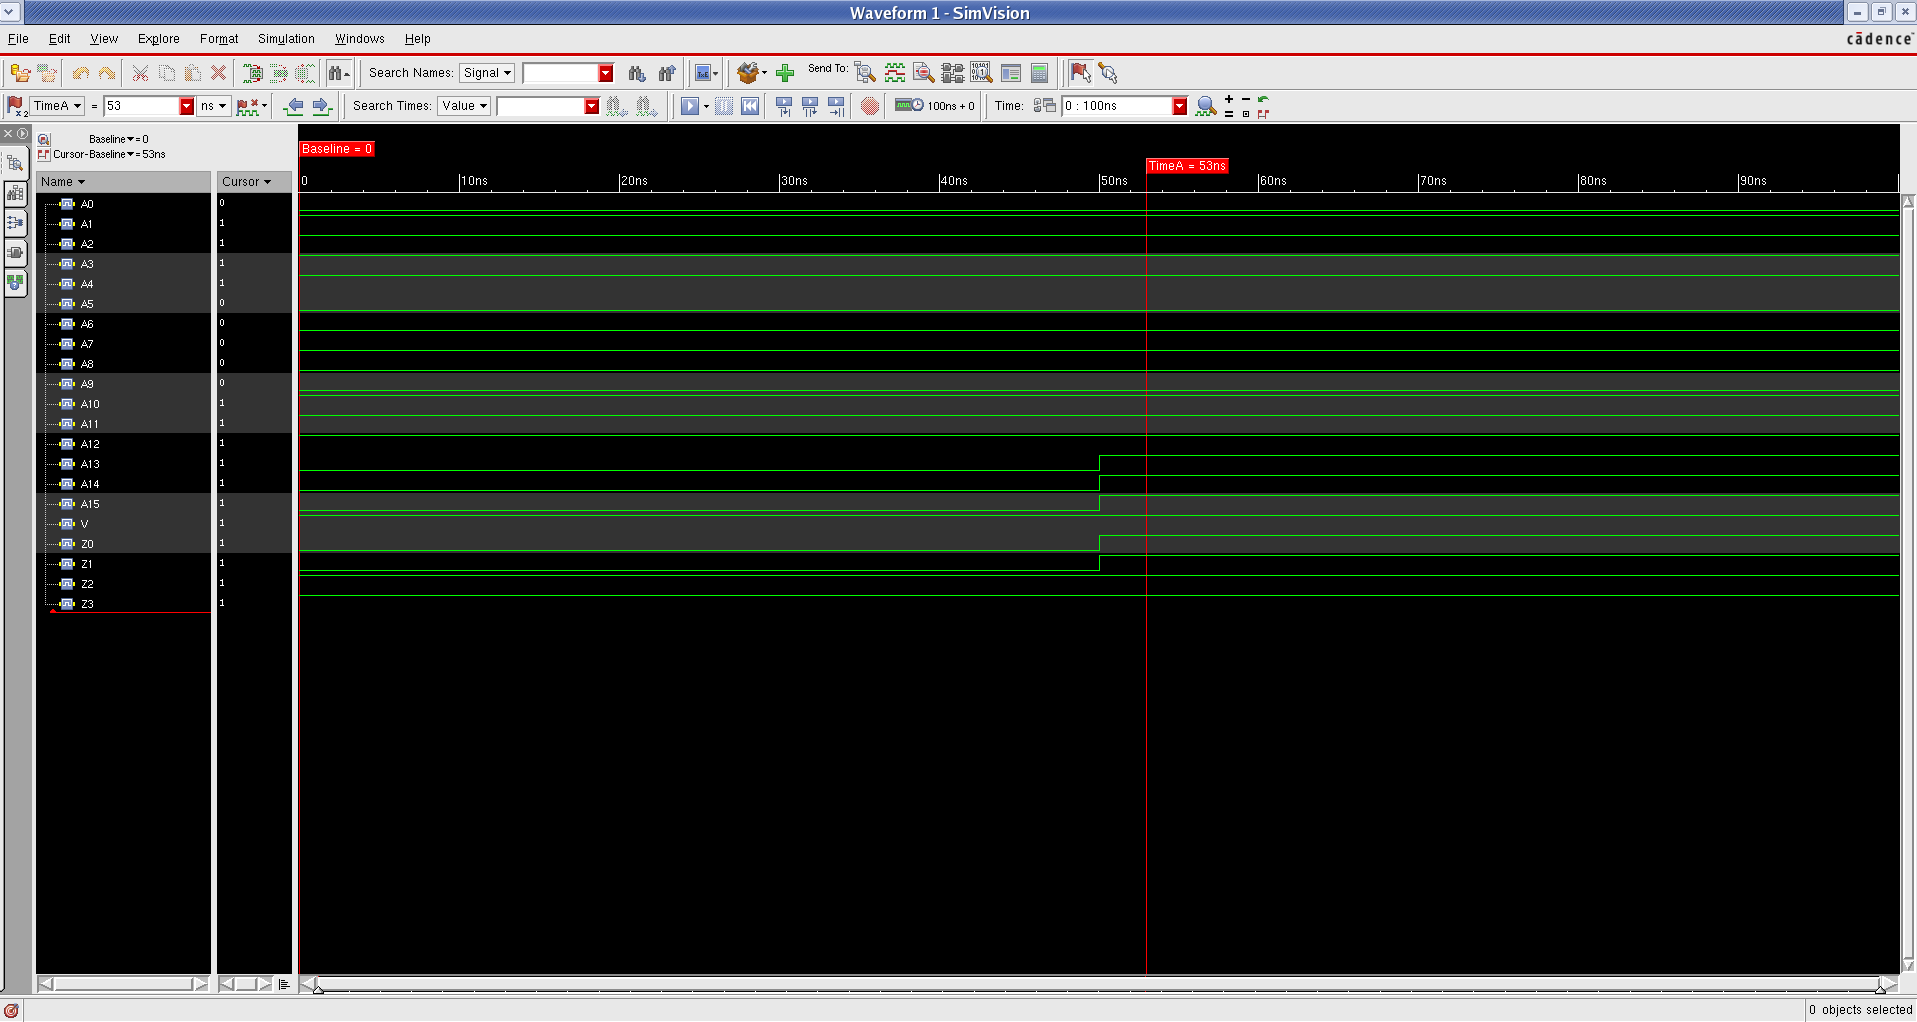
\includegraphics[width=0.9\textwidth]{chapter3/LZD16_nc}
\label{fig3.2b}
}
\caption{LZC单元的NC验证结果}
\label{fig3.2}
\end{figure}\\
\indent 最后,基于图\ref{fig2.3}所示的NORM指令的NC验证结果如图\ref{fig3.3}所示。表\ref{table3.1} 给出了LZC模块以及NORM指令模块的输入与输出的关系,其中LZC模块的输出为真实值的相反数,且在输入数的所有位全为0的时候,$V$也为0(实际值为1)。{\bfseries 从表\ref{table3.1}可以看出,图\ref{fig2.3}所示的NORM电路图可以正确的实现NORM指令的功能,即统计符号位后与符号位相同值的连续位数。}
\begin{table}[!hbpt]
\centering
\caption{LZC模块以及NORM模块的NC验证结果}
\label{table3.1}
\begin{tabular}{ccc}
\toprule
模块   & 输入   & 输出   \\
\midrule
\multirow{3}{*}{4-bit LZC} & 0100 & 10 \\
 & 1011 & 11 \\
 & 0000 & 00($V=0$) \\
\multirow{2}{*}{16-bit LZC} & 16'h1C1E & 1100  \\
& 16'hFC00 & 1111\\
\multirow{5}{*}{NORM模块} & 32'h0000\_FFFF& 32'h0000\_000F \\
& 32'hFFFF\_0000 & 32'h0000\_000F \\
& 32'h0F00\_0000 & 32'h0000\_0003 \\
& 32'h00F0\_0000 & 32'h0000\_0007 \\
& 32'hFF0F\_0000 & 32'h0000\_0007 \\

\bottomrule
\end{tabular}
\end{table}

对于NORM指令模块,输入(Src)为$32'hFFFF\_0000$和$32'h0000\_FFFF$时,输出(Lzc)是相同的,均为$32'h0000\_000F$,由于NORM指令的统计过程并不包括符号位在内,因此最终的结果为15而不是16,同理,输入为其它数值时也有类似结果。
\begin{figure}[!hbtp]
\centering
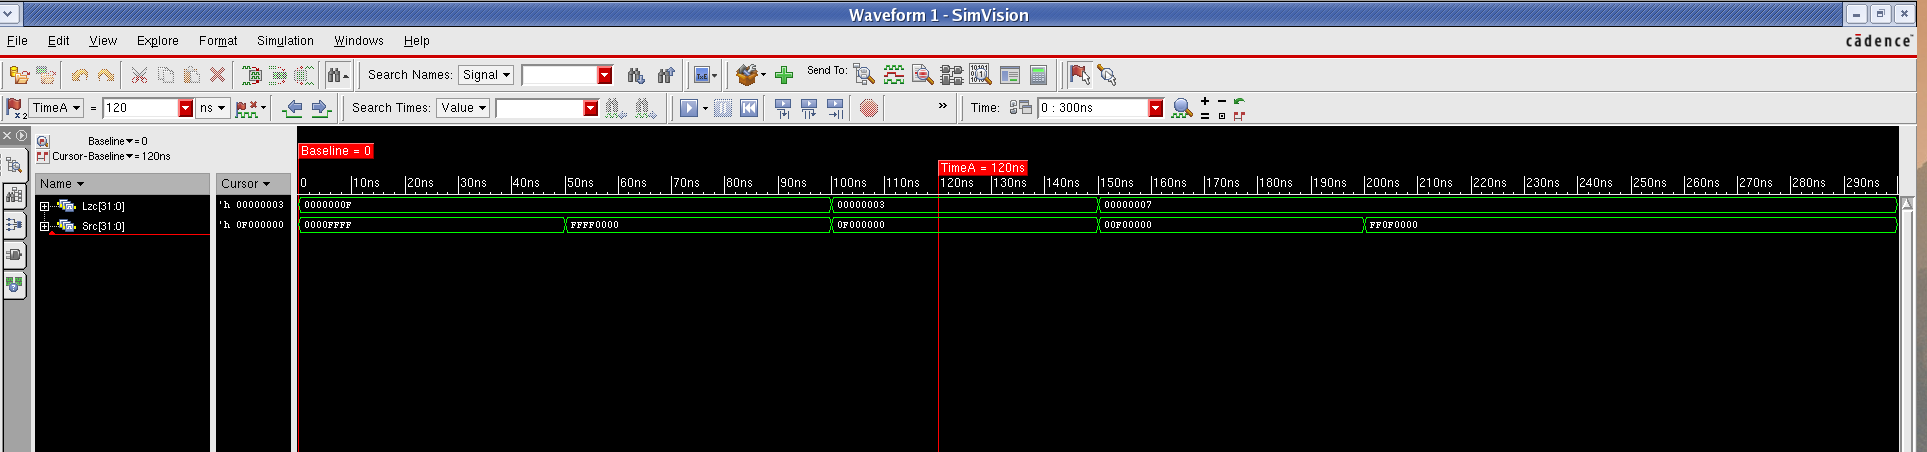
\includegraphics[width=0.9\textwidth]{chapter3/NORM_nc}
\caption{NORM模块NC验证结果}
\label{fig3.3}
\end{figure}

\chapter{时序分析与电路优化}
本章节主要对第二章设计的电路图导出.cdl网表借助HSpice工具软件进行时序分析,即输入到输出延时的大小的检测。
\section{工具简介}
HSPICE 是Meta-Software 公司为集成电路设计中的稳态分析,瞬态分析和频域分析等电路性能的模拟分析而开发的一个商业化通用电路模拟程序,它在伯克利的SPICE(1972 年推出),MicroSim公司的PSPICE (1984 年推出)以及其它电路分析软件的基础上,又加入了一些新的功能,经过不断的改进,目前已被许多公司、大学和研究开发机构广泛应用。

HSPICE 可与许多主要的EDA 设计工具,诸如Cadence,Workview 等兼容,能提供许多重要的针对集成电路性能的电路仿真和设计结果。采用HSPICE 软件可以在直流到高于100GHz 的微波频率范围内对电路作精确的仿真、分析和优化。在实际应用中, HSPICE能提供关键性的电路模拟和设计方案,并且应用HSPICE进行电路模拟时,其电路规模仅取决于用户计算机的实际存储器容量。

本次实验中需要对网表进行修改,相关原理主要参考文献\cite{bookHSpice2007},电子书版权为复旦大学所有。

\section{基于HSpice的时序结果}
在由Composer导出NORM模块的网表后,需要在网表中添加工艺库以及激励等信息,这两部分信息如下所示,首先确定.13的工艺库以及温度等参数。
\begin{verbatim}
0.13um INV Characteristics
.options LIST NODE POST
.lib 'l013_v2p5.lib' TT
.TEMP 25
.GLOBAL VDD, GND
OP
\end{verbatim}
下面是网表中输入的激励:
\begin{verbatim}
X Lzc<31> Lzc<30> Lzc<29> Lzc<28> Lzc<27> Lzc<26> Lzc<25>
+Lzc<24> Lzc<23> Lzc<22> Lzc<21> Lzc<20> Lzc<19> Lzc<18> Lzc<17> Lzc<16>
+Lzc<15> Lzc<14> Lzc<13> Lzc<12> Lzc<11> Lzc<10> Lzc<9> Lzc<8> Lzc<7> Lzc<6>
+Lzc<5> Lzc<4> Lzc<3> Lzc<2> Lzc<1> Lzc<0> Src<31> src1<30> src1<29>
+Src<28> Src<27> Src<26> Src<25> Src<24> Src<23> Src<22> Src<21>
+Src<20> Src<19> Src<18> Src<17> Src<16> Src<15> Src<14> Src<13>
+Src<12> Src<11> Src<10> Src<9> Src<8> Src<7> Src<6> Src<5> Src<4>
+Src<3> Src<2> Src<1> Src<0> 
+NORM
V1 VDD 0 1.2V
V4 Src<31> 0 0
V5 Src<30> 0 0
V6 Src<29> 0 0
V7 Src<28> 0 pulse(0 1.2V 0.5N 0N 0N 2N 4N) 
V8 Src<27> 0 1.2V
V9 Src<26> 0 1.2V 
V10 Src<25> 0 1.2V 
V11 Src<24> 0 1.2V 
V12 Src<23> 0 0
V13 Src<22> 0 0
V14 Src<21> 0 0 
V15 Src<20> 0 0
V16 Src<19> 0 0
V17 Src<18> 0 0 
V18 Src<17> 0 0 
V19 Src<16> 0 0 
V20 Src<15> 0 0
V21 Src<14> 0 0
V22 Src<13> 0 0
V23 Src<12> 0 0
V24 Src<11> 0 1.2V
V25 Src<10> 0 0
V26 Src<9> 0 1.2V 
V27 Src<8> 0 1.2V 
V28 Src<7> 0 1.2V 
V29 Src<6> 0 1.2V 
V30 Src<5> 0 1.2V 
V31 Src<4> 0 1.2V 
V32 Src<3> 0 1.2V 
V33 Src<2> 0 1.2V
V34 Src<1> 0 1.2V 
V35 Src<0> 0 1.2V
.tran 0.2n 10n
.end
\end{verbatim}
根据NORM指令的具体功能,在输入端口Src<28>输入周期为4ns的脉冲瞬态电压源,脉冲宽度为2ns。定义电压脉冲源的具体语法如下所示:
\begin{verbatim}
Vxxx n+ n- PU<LSE> <(>v1 v2 <td <tr <tf <pw <per>>>>>  <)>
\end{verbatim}
其中\verb|< >|为可省略部分。.trans 0.2n 10n表示工具共需要分析10ns的瞬态分析,步长为0.2ns。

最后,HSpice的时序分析结果如图\ref{fig4.1}所示。从图中可以看出,当输入为最高5位(包括符号位)由00001变为00011时,输出的最低两位由11变为10,其输出延时为395ps(如图所示),同时,输出随输入的变化情况与NC的仿真波形都说明设计的NORM指令模块功能的正确性!
\begin{figure}[!hbtp]
\centering
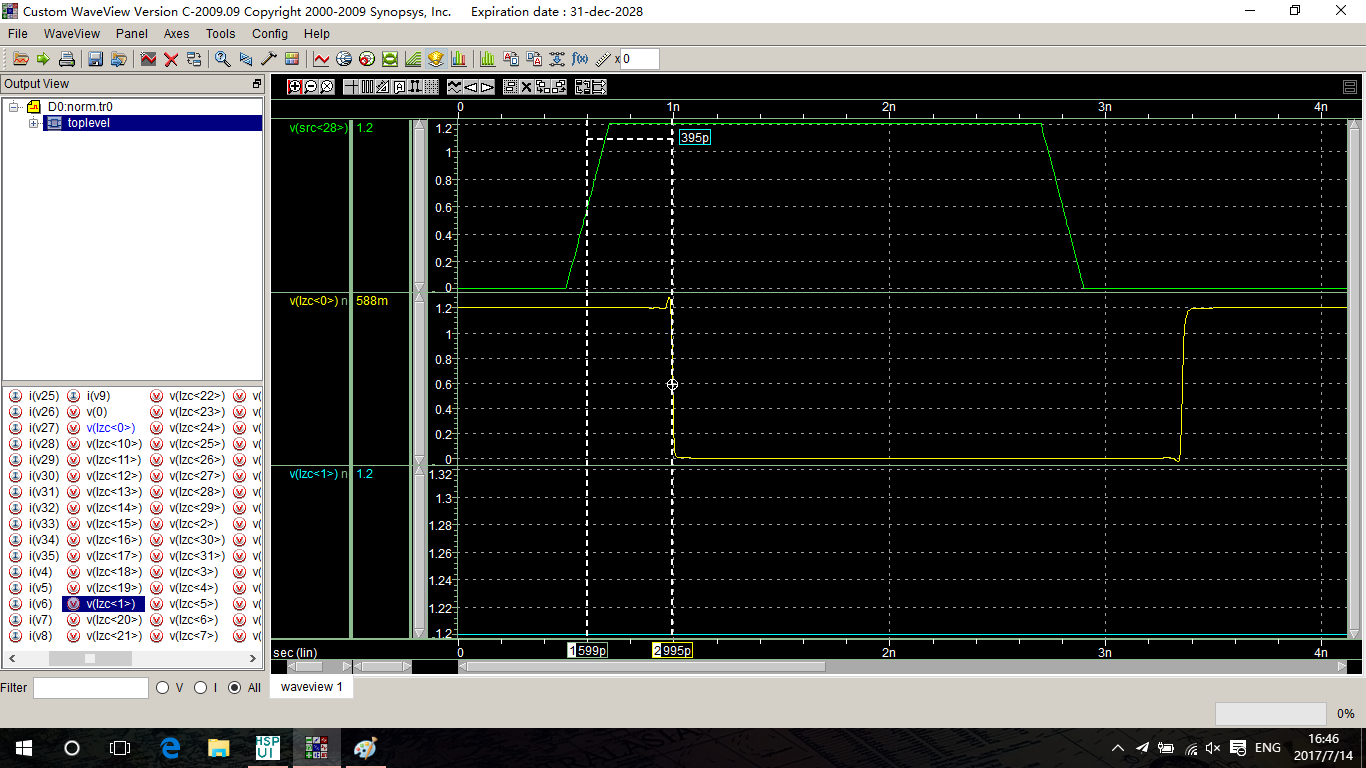
\includegraphics[width=0.9\textwidth]{chapter4/NORM_HSPICE_1}
\caption{NORM指令的HSpice分析结果}
\label{fig4.1}
\end{figure}


\chapter{版图设计与验证}
本章节主要给出NORM指令基于第二章电路图的版图设计,包括电路图中的所有模块的版图设计,并对最终的设计进行DRC、LVS检查。
为了控制篇幅,这里仅给出所有子模块中几个主要模块的版图、DRC验证结果、LVS验证结果的截图。

{
\itshape
\bfseries
需要指出的是,在完成版图设计过程中,为了方便电源、地的走线,基本单元的高度被设置为同样的高度;为了减少需要的金属层,在连线过程中采取的基本原则是:横向采用M1层金属,纵向连线采用M2层金属,这样有利于减少不必要的绕线,因此,本次NORM的设计所有的连线都在M1、M2层内完成,没用到高层金属,但这样也导致设计中需要的M1、M2层间的通孔数量较多;最后,为了实现NORM指令最终的版图尽可能更规则,2路31位选择器采用双列的形式实现,这样就可以保证NORM模块最终可实现近似正方形的版图。
}

下面对几个主要模块进行说明,包括版图、DRC验证结果以及LVS验证结果。

\subsubsection{AND2模块}
本模块主要完成量输入与门的设计。其版图、DRC检查结果、LVS检查结果如图\ref{fig5.1}所示。
\begin{figure}[!hbtp]
\centering
\subfigure[AND2版图]{
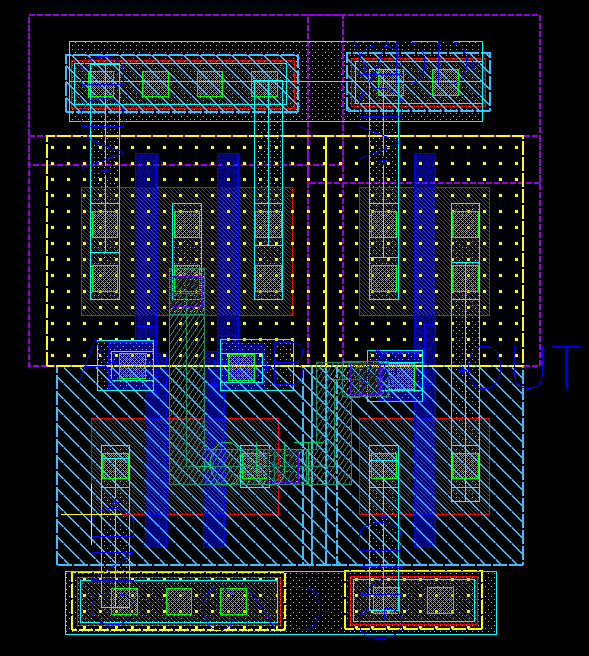
\includegraphics[width=0.7\textwidth]{chapter5/AND2}
\label{fig5.1a}
}
\subfigure[AND2 DRC验证结果]{
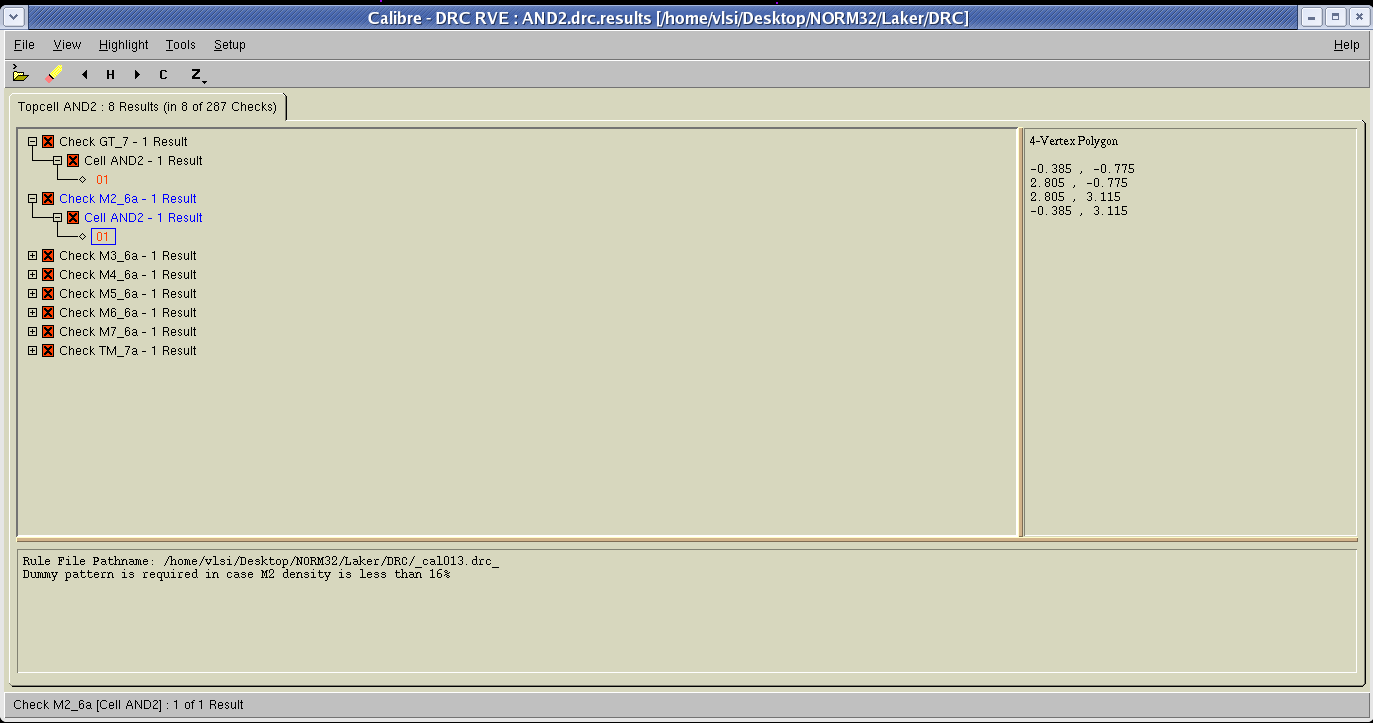
\includegraphics[width=0.7\textwidth]{chapter5/AND2_drc}
\label{fig5.1b}
}
\subfigure[AND2 LVS验证结果]{
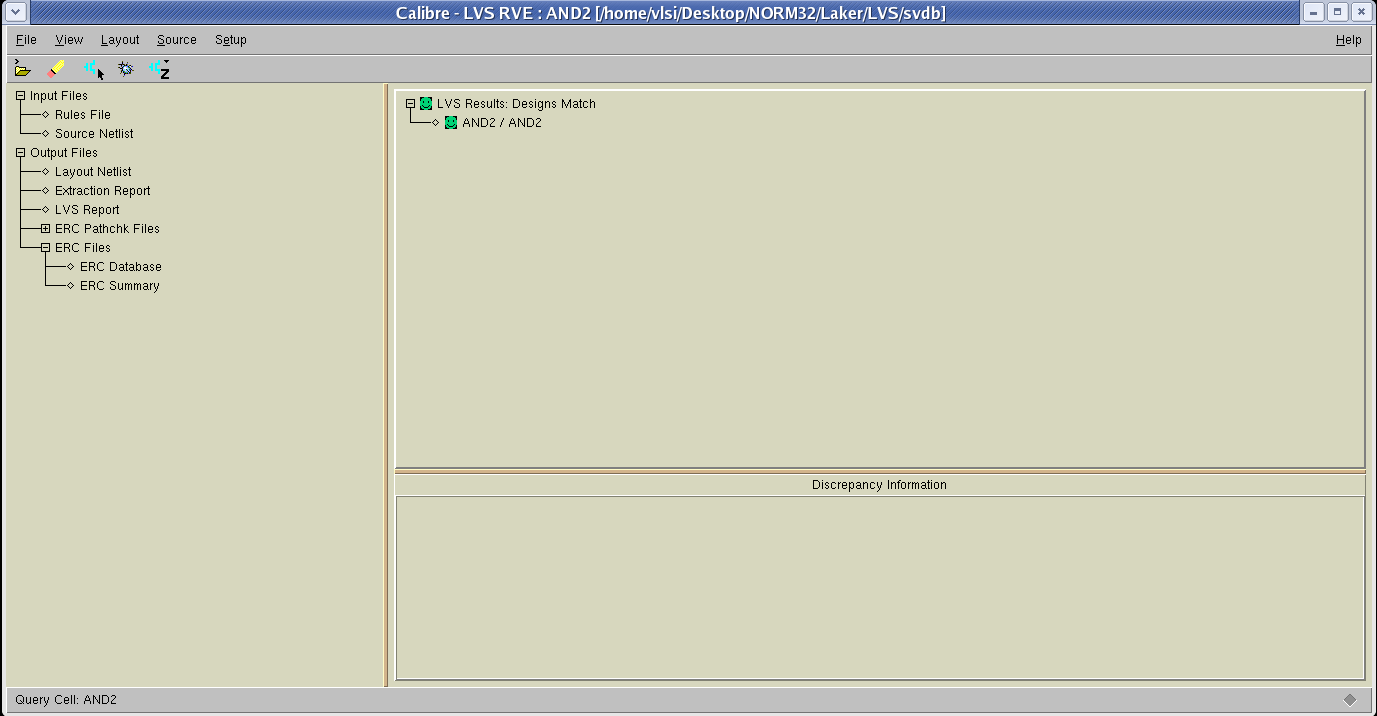
\includegraphics[width=0.7\textwidth]{chapter5/AND2_lvs}
\label{fig5.1c}
}
\caption{AND2版图设计及其验证结果}
\label{fig5.1}
\end{figure}
\subsubsection{IAO模块}
本模块主要完成三输入与或逻辑,即输入A与B,然后其结果再与C进行或操作。模块的版图等结果如图\ref{fig5.2}所示。
\begin{figure}[!hbtp]
\centering
\subfigure[IAO模块版图]{
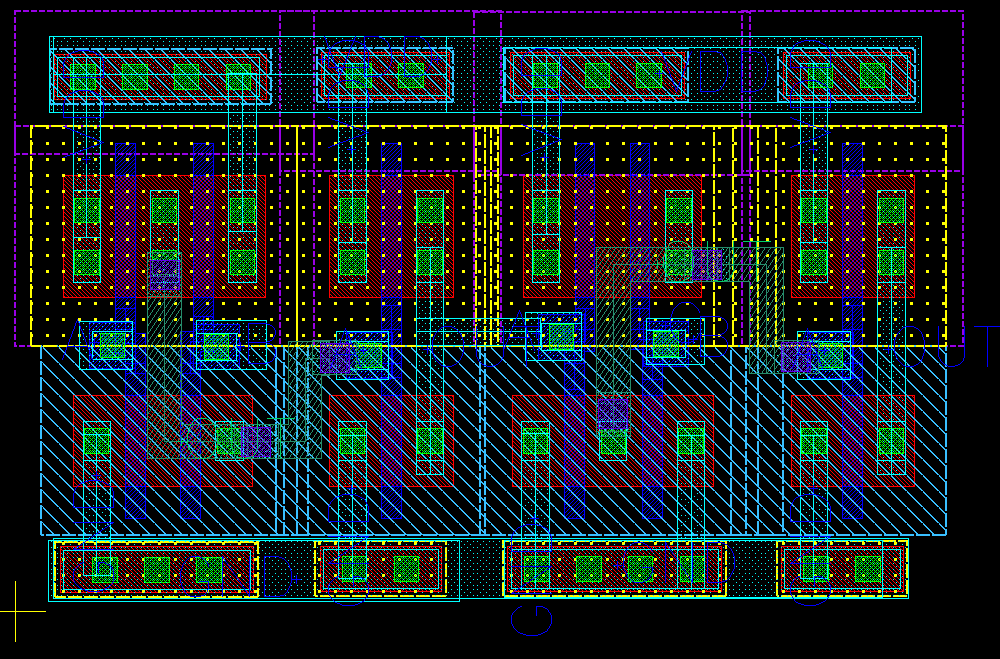
\includegraphics[width=0.7\textwidth]{chapter5/IAO}
\label{fig5.2a}
}
\subfigure[IAO DRC验证结果]{
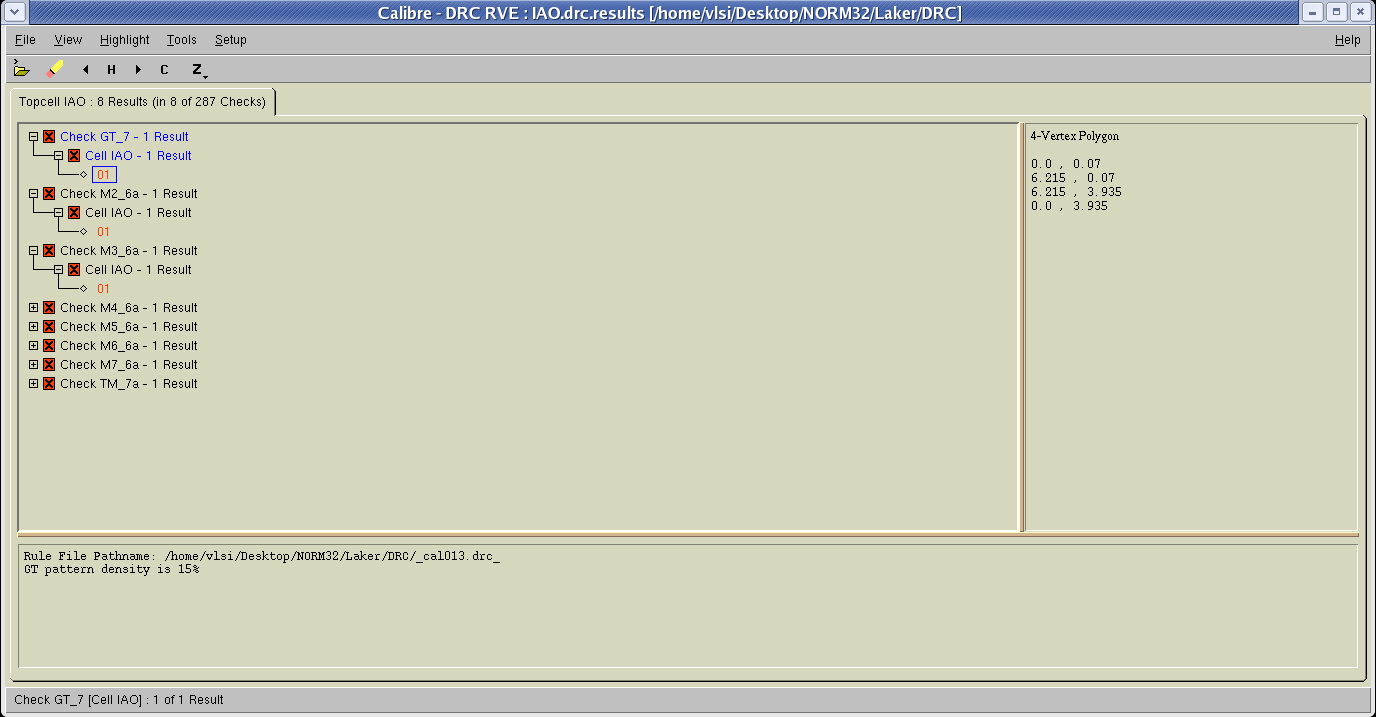
\includegraphics[width=0.7\textwidth]{chapter5/IAO_drc}
\label{fig5.2b}
}
\subfigure[IAO LVS验证结果]{
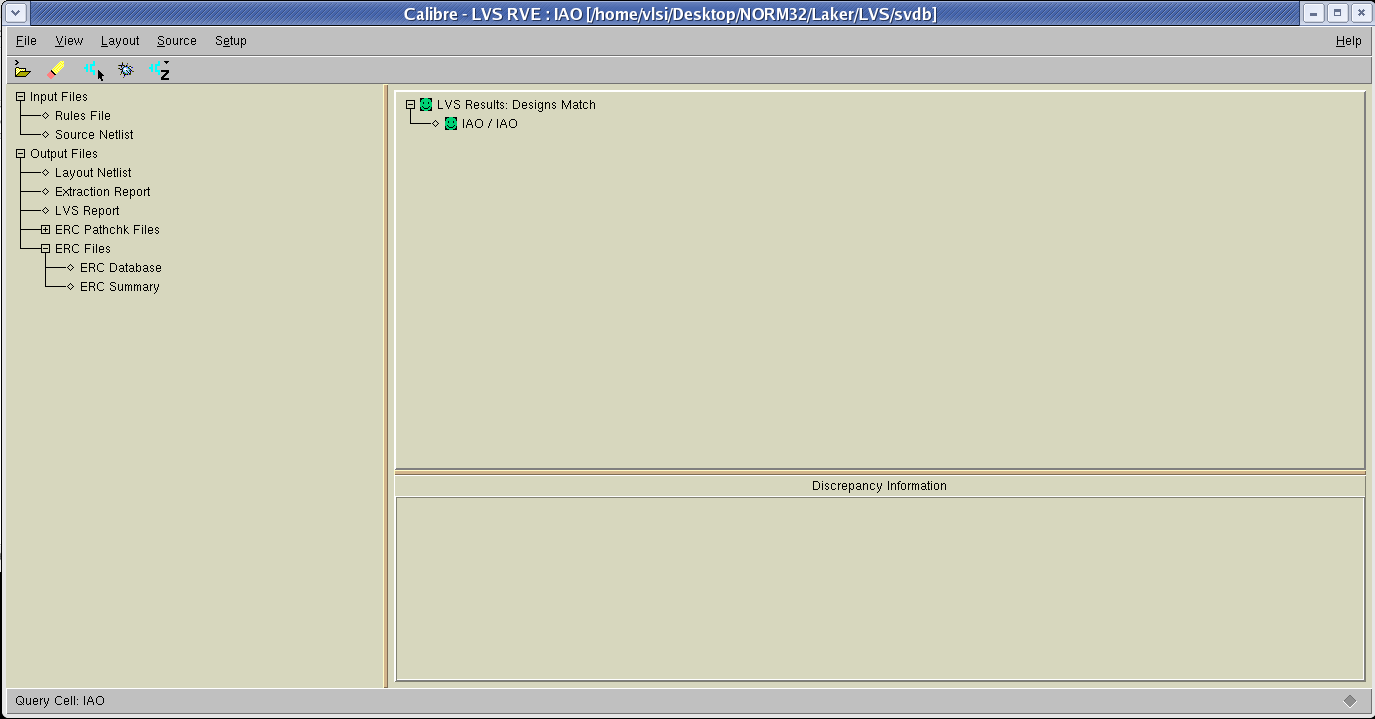
\includegraphics[width=0.7\textwidth]{chapter5/IAO_lvs}
\label{fig5.2c}
}
\caption{IAO版图设计及其验证结果}
\label{fig5.2}
\end{figure}
\subsubsection{MUX2\_1模块}
本模块主要完成两路一位选择器的功能,其结果如图\ref{fig5.3}所示,为防止出现有源区距离过小的DRC错误,其各个顶层单元之间的有源区彼此重合。
\begin{figure}[!hbtp]
\centering
\subfigure[MUX2\_1模块版图]{
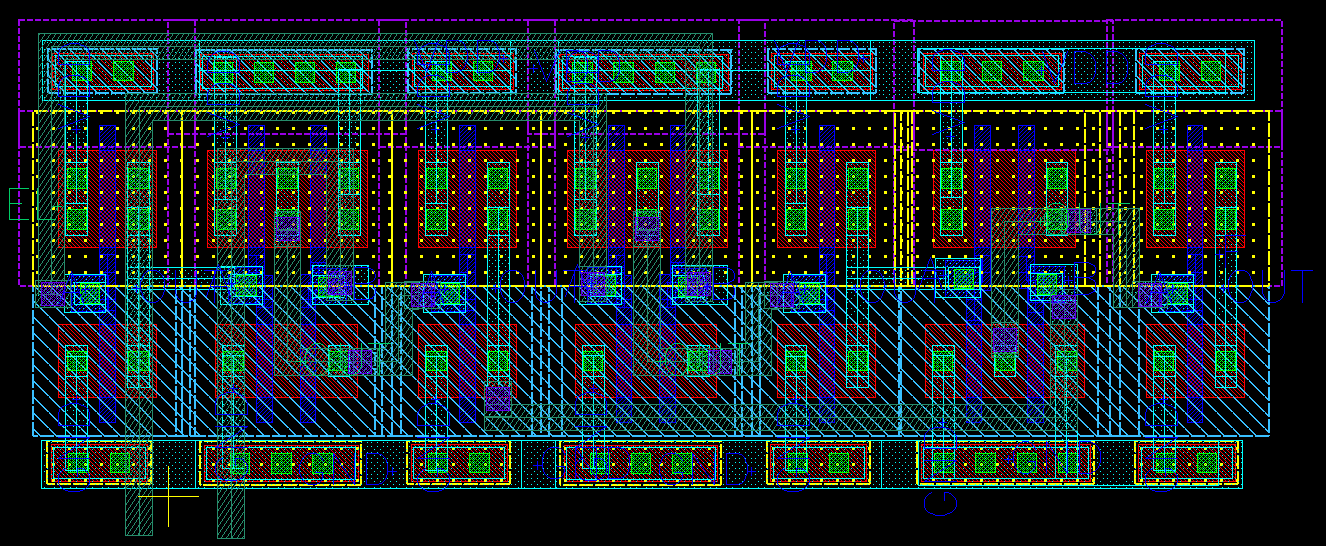
\includegraphics[width=0.7\textwidth]{chapter5/MUX2_1}
\label{fig5.3a}
}
\subfigure[MUX2\_1 DRC验证结果]{
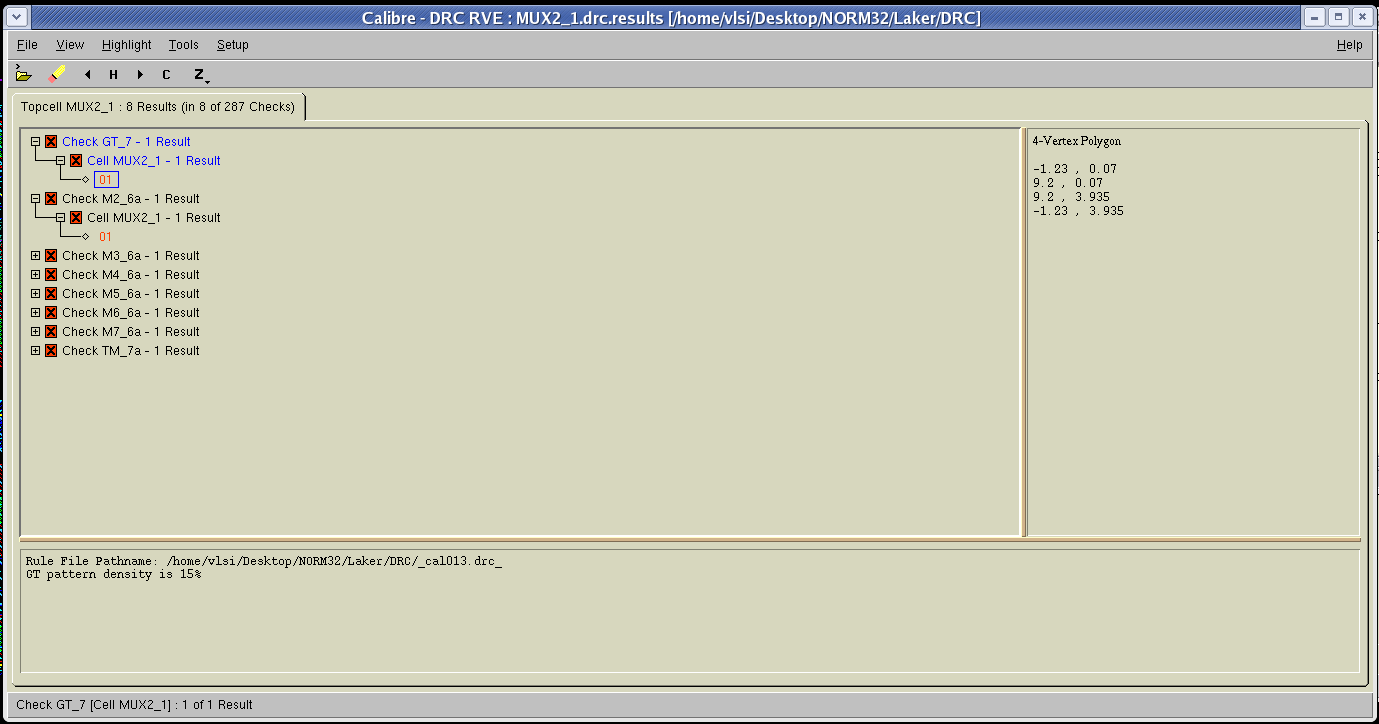
\includegraphics[width=0.7\textwidth]{chapter5/MUX2_1_drc}
\label{fig5.3b}
}
\subfigure[MUX2\_1 LVS验证结果]{
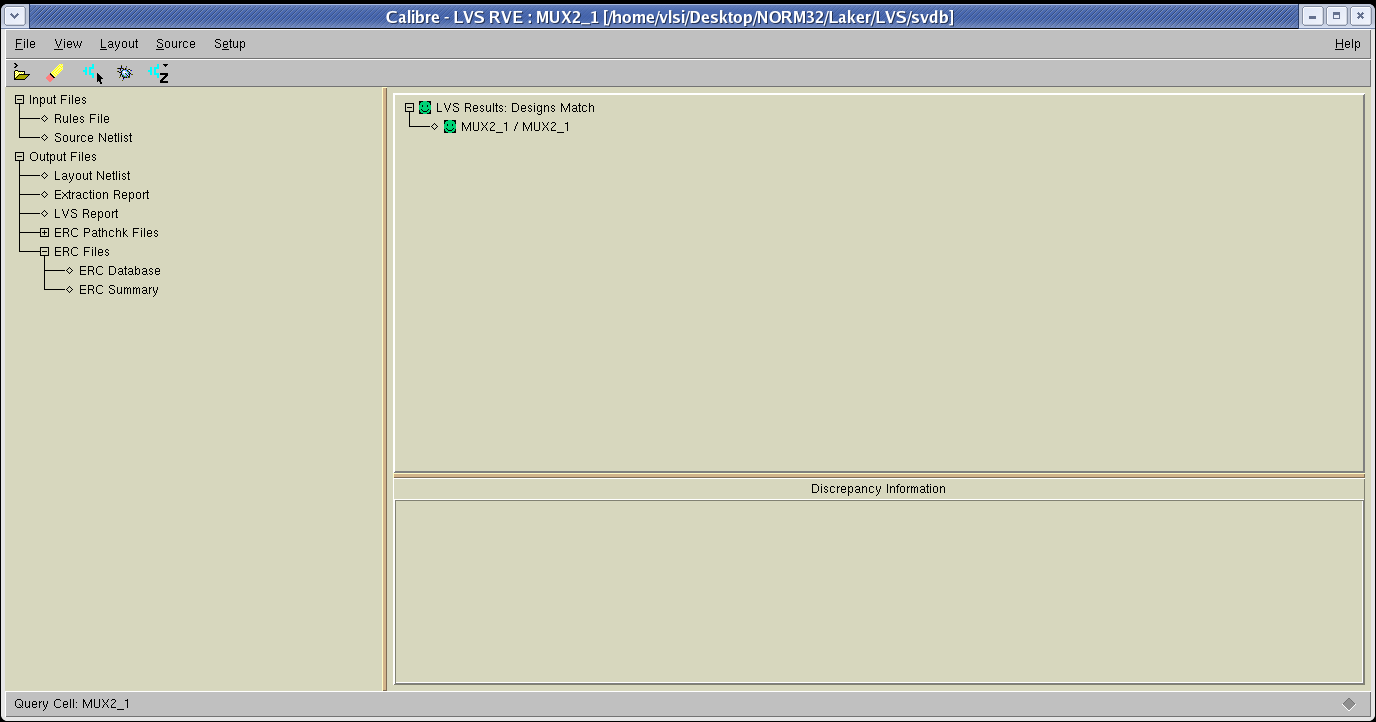
\includegraphics[width=0.7\textwidth]{chapter5/MUX2_1_lvs}
\label{fig5.3c}
}
\caption{MUX2\_1版图设计及其验证结果}
\label{fig5.3}
\end{figure}
\subsubsection{LZD4模块}
本模块完成4-bit输入数据的前导零检测功能,输出为2位,且真实结果为输出的反向。其结果如图\ref{fig5.4}所示。
\begin{figure}[!hbtp]
\centering
\subfigure[LZD4模块版图]{
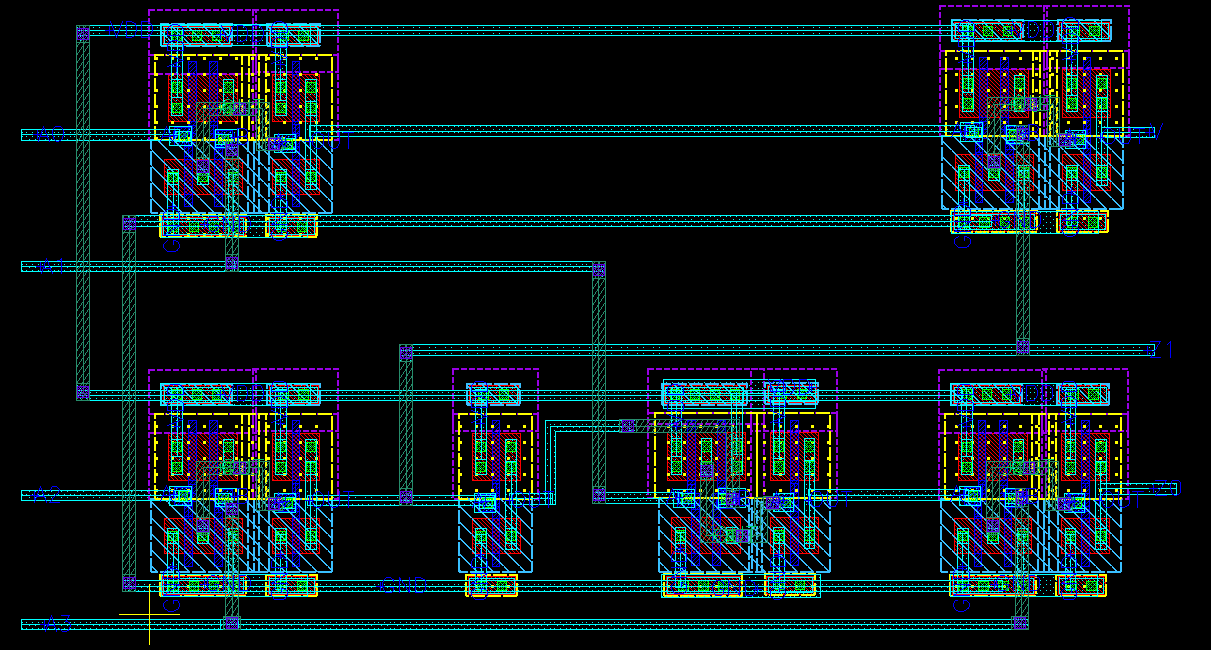
\includegraphics[width=0.7\textwidth]{chapter5/LZD4}
\label{fig5.4a}
}
\subfigure[LZD4 DRC验证结果]{
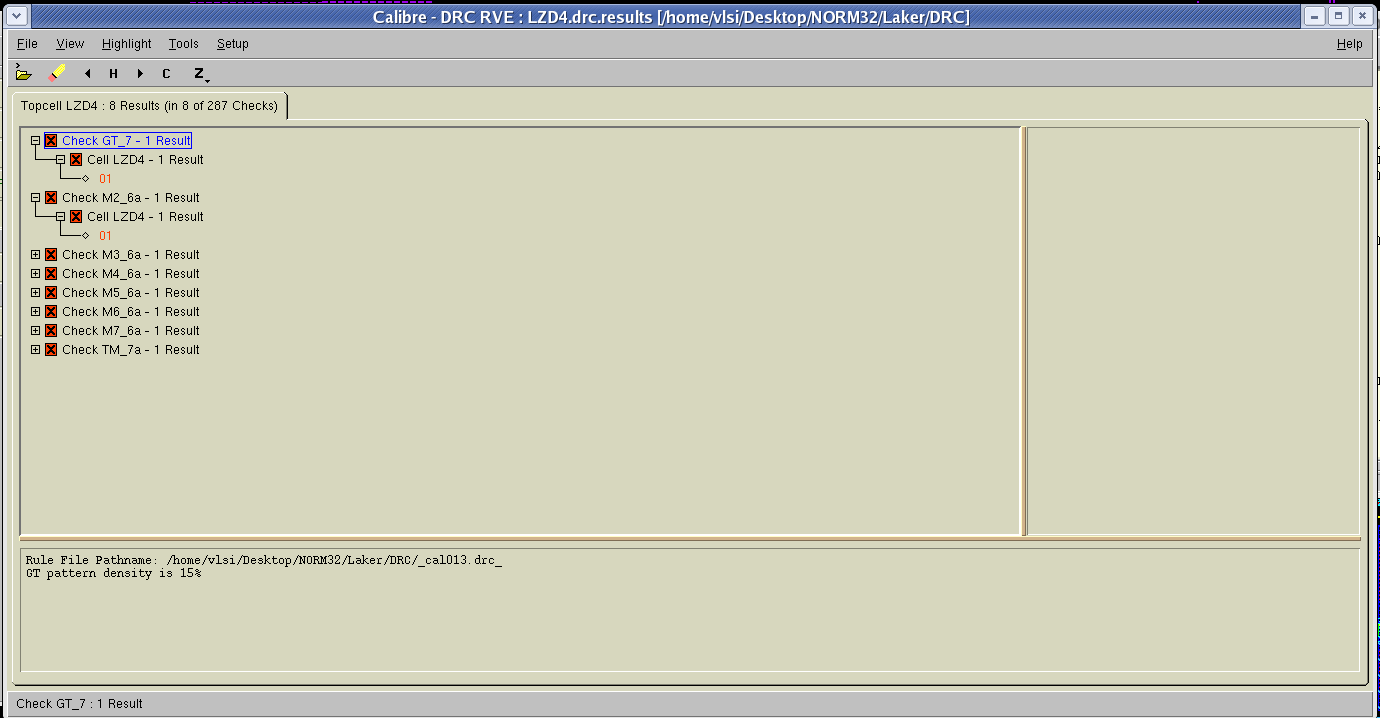
\includegraphics[width=0.7\textwidth]{chapter5/LZD4_drc}
\label{fig5.4b}
}
\subfigure[LZD4 LVS验证结果]{
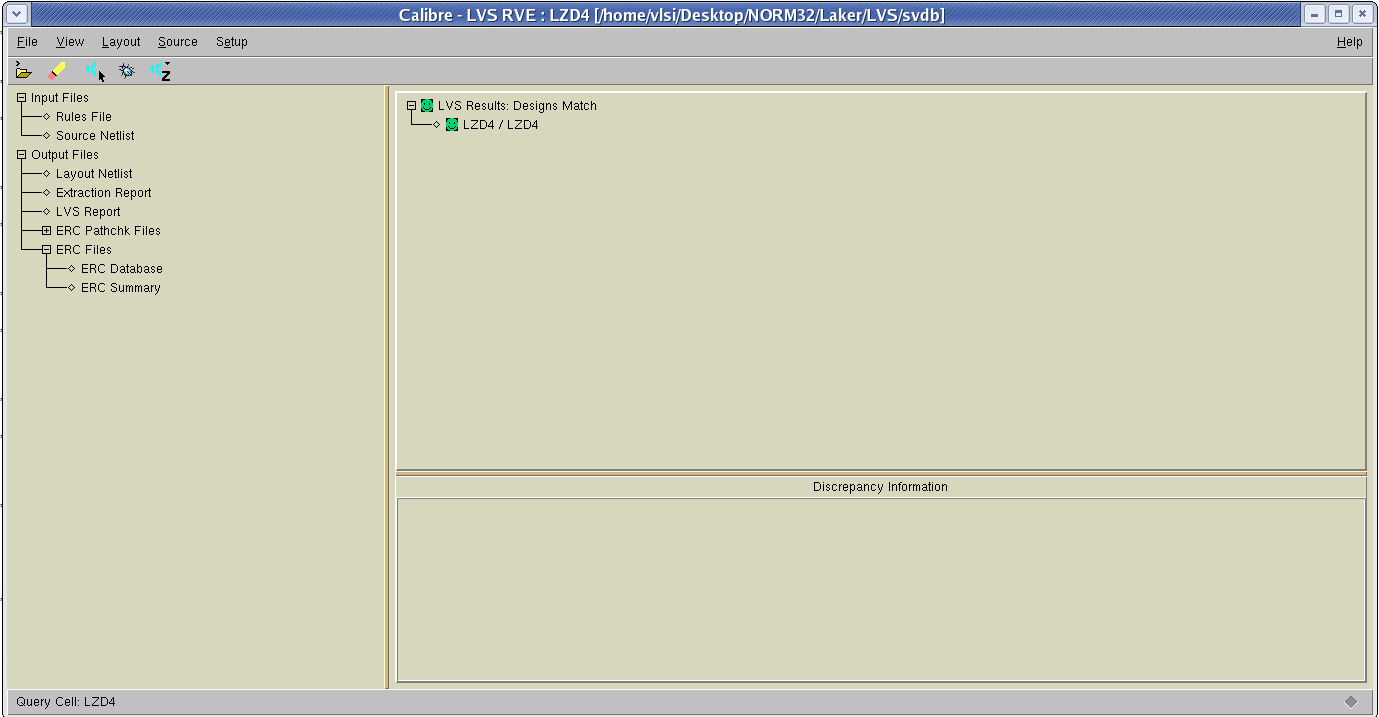
\includegraphics[width=0.7\textwidth]{chapter5/LZD4_lvs}
\label{fig5.4c}
}
\caption{LZD4版图设计及其验证结果}
\label{fig5.4}
\end{figure}
\subsubsection{LZD16模块}
本模块在LZD8(省略)的基础上完成16-bit输入数据的前导零计算功能,其输出同样为真实结果的反向,结果如图\ref{fig5.5}所示。
\begin{figure}[!hbtp]
\centering
\subfigure[LZD16模块版图]{
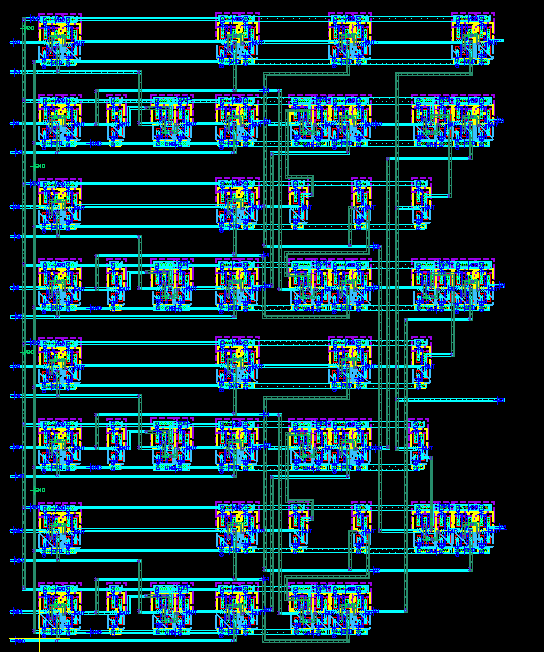
\includegraphics[width=0.7\textwidth]{chapter5/LZD16}
\label{fig5.5a}
}
\subfigure[LZD16 DRC验证结果]{
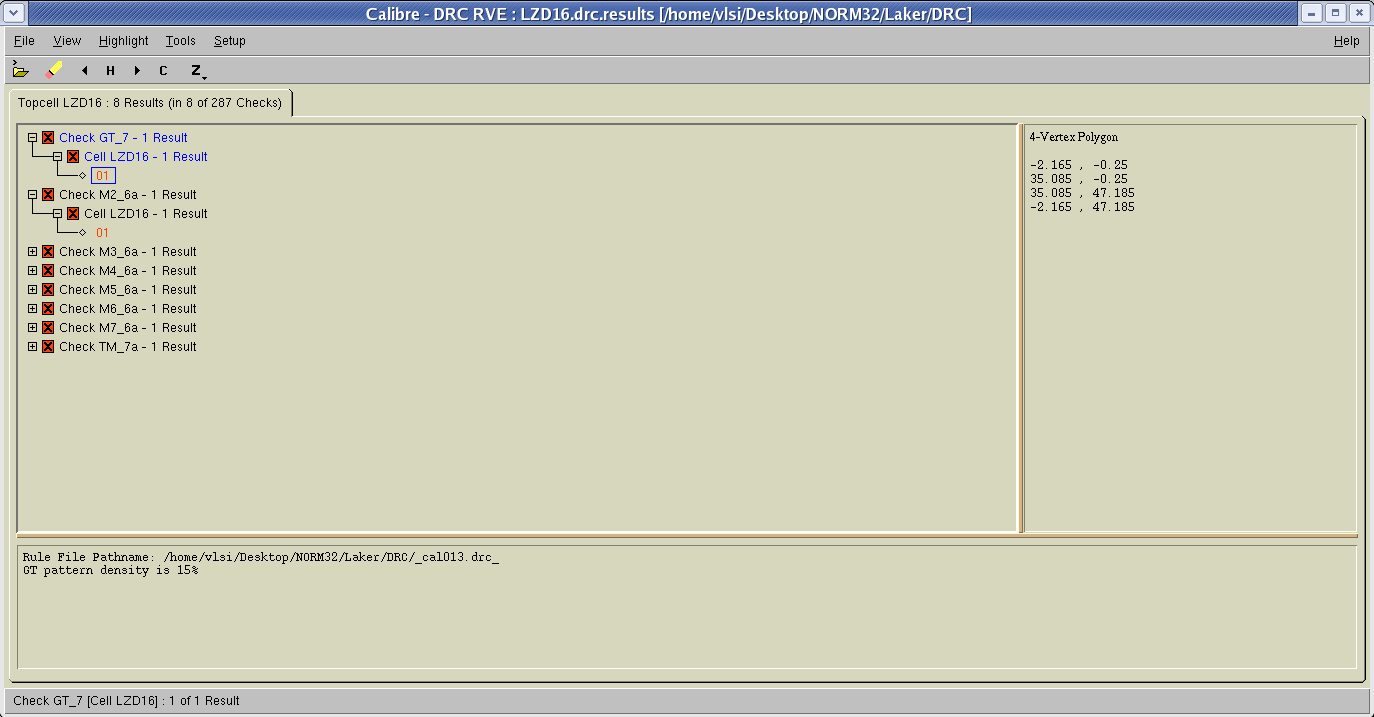
\includegraphics[width=0.7\textwidth]{chapter5/LZD16_drc}
\label{fig5.5b}
}
\subfigure[LZD16 LVS验证结果]{
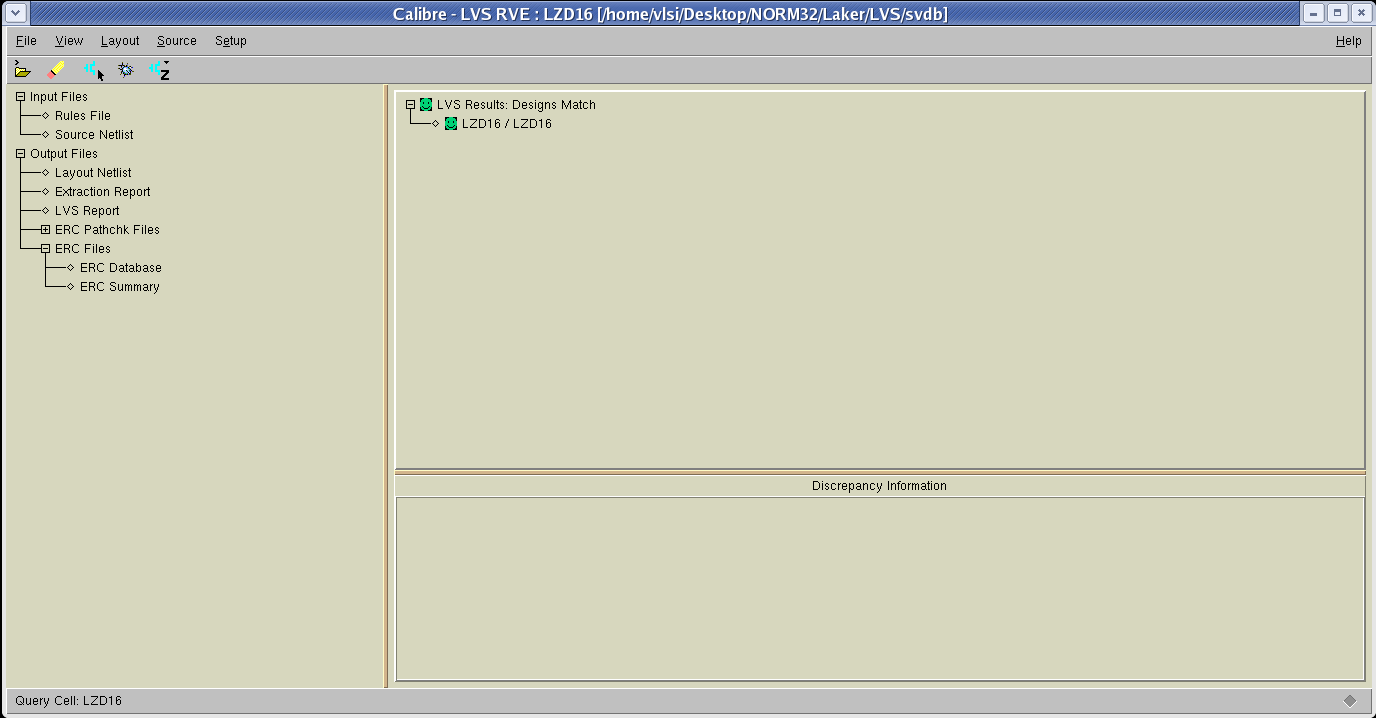
\includegraphics[width=0.7\textwidth]{chapter5/LZD16_lvs}
\label{fig5.5c}
}
\caption{LZD16版图设计及其验证结果}
\label{fig5.5}
\end{figure}

\subsubsection{LZDF模块}
本模块(LZDF: LZD Final)在LZD16的基础上完成32-bit输入数据的前导零计算功能,其输出同样为真实结果的反向,此外,其输入数据也由以前的直接输入变为从选择器输入,而两路选择器的输入,一路为未处理的输入数据,另一路为按位取反输入数据的结果,选择信号为输入数据的符号位。结果如图
\ref{fig5.6}所示。
\begin{figure}[!hbtp]
\centering
\subfigure[LZDF模块版图]{
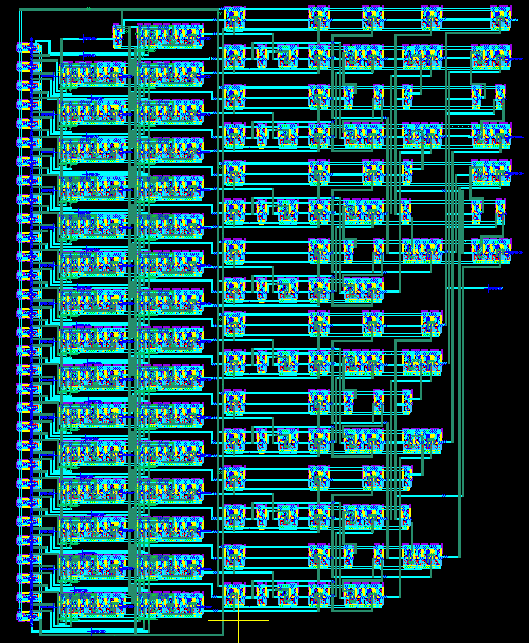
\includegraphics[width=0.6\textwidth]{chapter5/LZDF}
\label{fig5.6a}
}
\subfigure[LZDF DRC验证结果]{
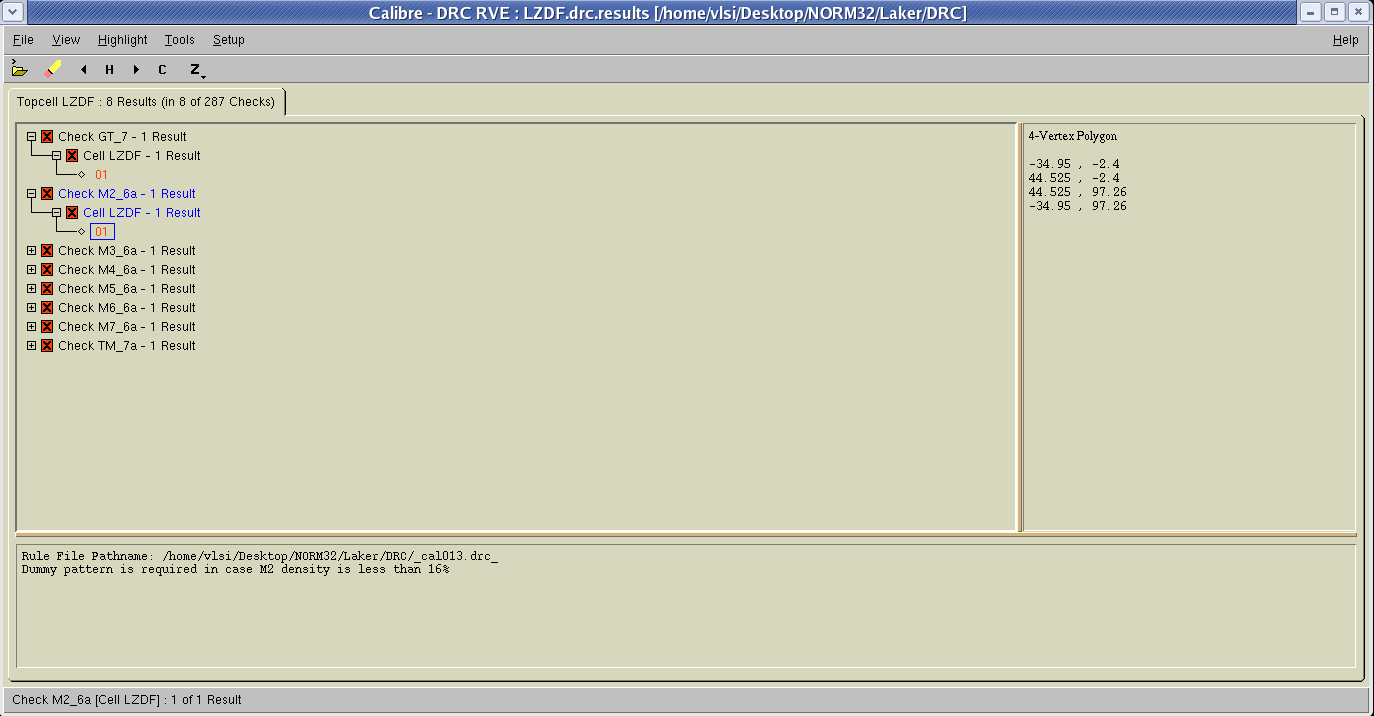
\includegraphics[width=0.7\textwidth]{chapter5/LZDF_drc}
\label{fig5.6b}
}
\subfigure[LZDF LVS验证结果]{
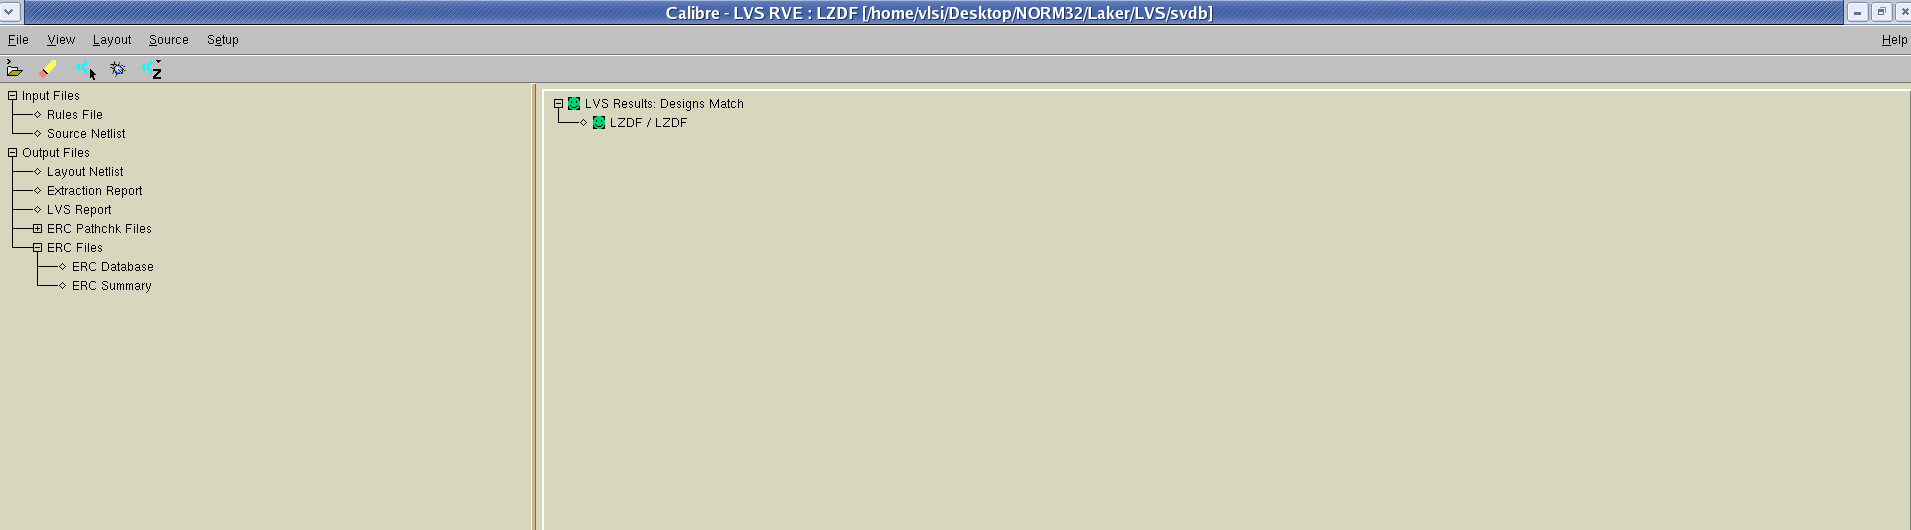
\includegraphics[width=0.7\textwidth]{chapter5/LZDF_lvs}
\label{fig5.6c}
}
\caption{LZDF版图设计及其验证结果}
\label{fig5.6}
\end{figure}
\subsubsection{NORM模块}
最后,本模块在LZDF模块的基础上,完成NORM指令模块的版图设计,其输出为32位,其中高位(31$\sim$5恒为0)。其结果如图\ref{fig5.7}所示。
\begin{figure}[!hbtp]
\centering
\subfigure[NORM模块版图]{
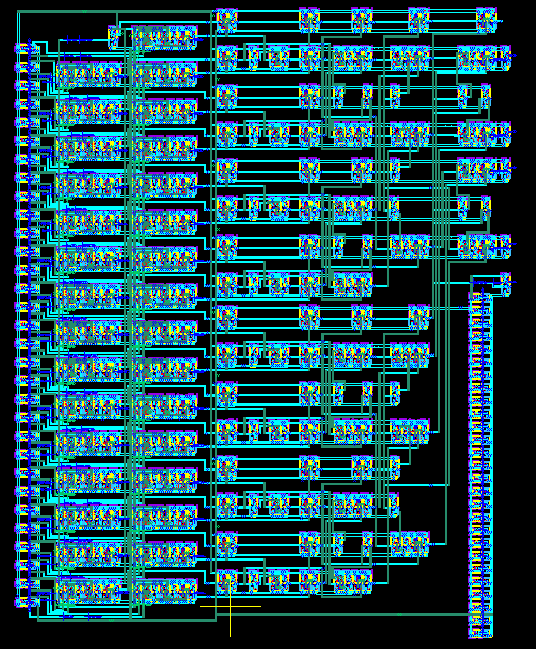
\includegraphics[width=0.7\textwidth]{chapter5/NORM}
\label{fig5.7a}
}
\subfigure[NORM DRC验证结果]{
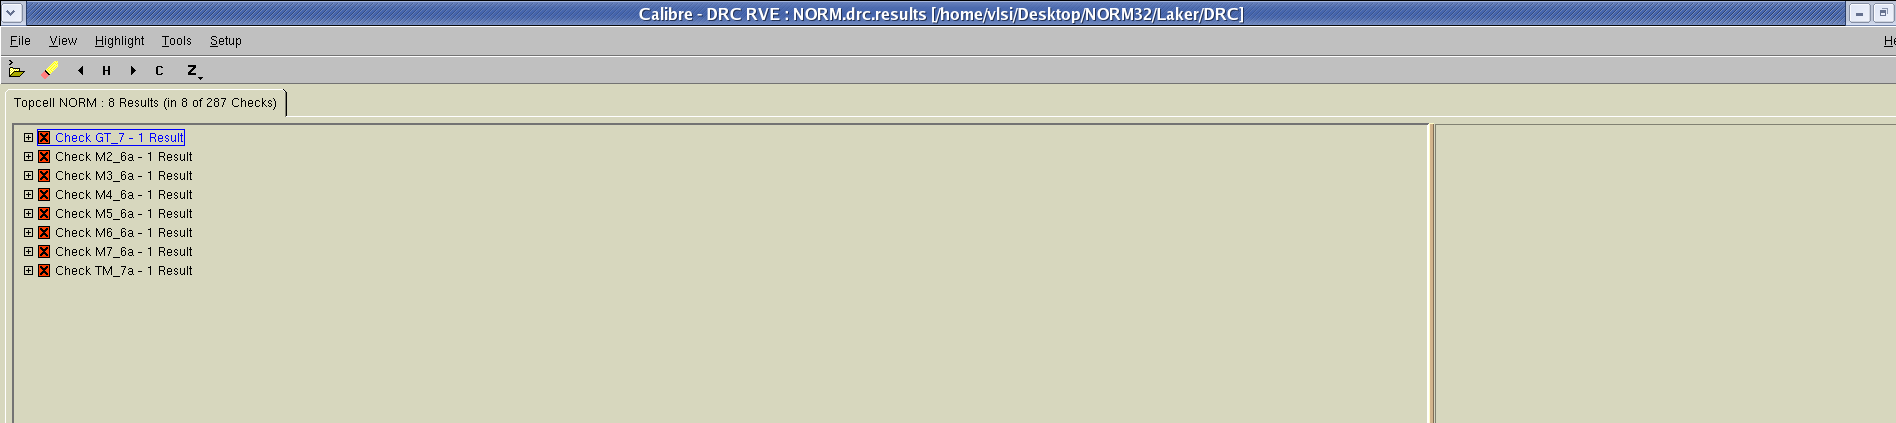
\includegraphics[width=0.7\textwidth]{chapter5/NORM_drc}
\label{fig5.7b}
}
\subfigure[NORM LVS验证结果]{
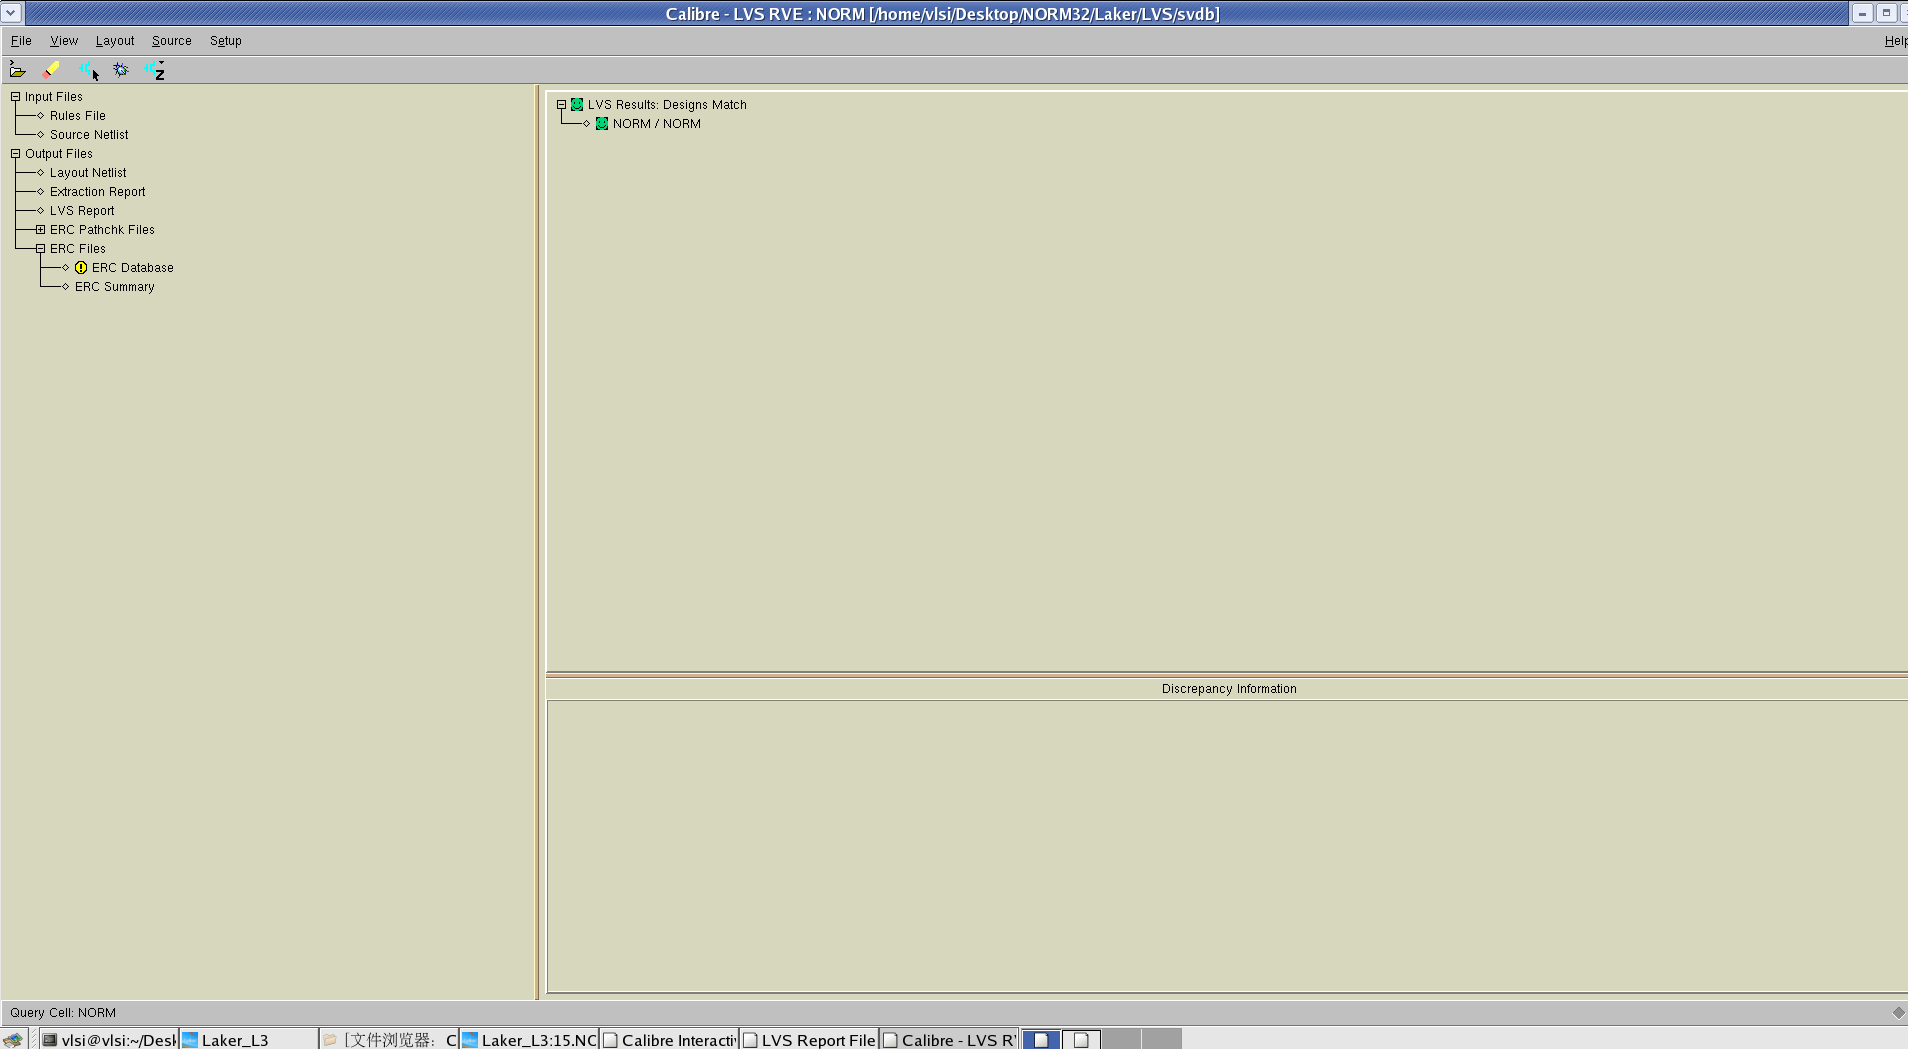
\includegraphics[width=0.7\textwidth]{chapter5/NORM_lvs}
\label{fig5.7c}
}
\caption{NORM 版图设计及其验证结果}
\label{fig5.7}
\end{figure}

\chapter{实验总结}
通过完成本次实验,熟悉了数字电路全定制流程,包括最初的功能分析、电路图设计、功能验证、时序分析与优化以及后来的版图设计以及DRC、LVS验证等。实验结果表明,设计的NORM指令模块可以实现正确的功能(NC、HSpice结果),输入至输出的响应延时为395ps(HSpice结果),且版图设计与电路图设计一致、没有DRC错误(通过DRC、LVS验证)。下面对本次实验进行总结。
\section{试验中遇到的问题与解决办法}
回顾整个实验流程,遇到的几个主要问题及其解决办法如下:
\begin{itemize}
\item \textbf{由Composer导出电路图的NC-Verilog文件以及.cdl网表过程中,导出失败} \\
\textbf{解决办法:}通过对导出文件的过程进行分析,发现在导出顶层模块的上述文件时,需要首先将顶层模块包含的所有底层模块的上述文件导出,然后即可解决错误。
\item \textbf{在基于设计的.cdl网表进行时序分析时,输出并不会跟随输入变化}\\
\textbf{解决办法:}通过.sp文件中瞬态源的周期得以解决,即将在Src<27>输入端口的脉冲源的周期由最开始的2ns增加为4ns,同时将高电平维持时间由原来的1ns改为2ns后,输出正常,其结果见图\ref{fig4.1}。
\item \textbf{版图设计中DRC验证出现问题} \\
\textbf{解决办法:}一般发生DRC违反,主要由版图设计中存在电器规则违反所致,如金属层之间的间距过小、金属的面积过小等错误。根据提示修改这些错误后,所有模块均通过DRC检查。
\item \textbf{版图设计中LVS验证出现问题}\\
\textbf{解决办法:}一般发生LVS错误,可以是.cdl文件与.gds文件之间存在不一致导致,包括版图中器件的尺寸与电路图中器件的尺寸或名字不一致、连线存在错误等。经过对.cdl文件以及版图中不一致的地方进行修改后,所有模块的LVS检查均通过验证。
\end{itemize}
\section{实验收获与不足}
从这一次实验中熟悉了各种全定制工具的使用,对于Virtuoso工具的使用更加熟练,对于版图设计规则有了更全的认识,能够较好的运用工具来实现设计,对全定制设计有了更全面的理解。

通过完成tms320 DSP的NORM指令的全定制,对实际数字电路功能的实现有了更深的理解,包括功能分析以及具体电路的设计等,为以后的工作打下了坚实的基础。在电路设计过程中,学习了如何通过阅读论文来找出比较有效的解决方案,更重要的,通过完成低功耗的LZC模块,了解了一种低功耗设计思路,即通过逻辑优化以及器件共享来减少所需的器件的数量,从而降低电路的整体功耗。

在这段时间里部分完成NORM指令的全定制设计,自己动手实践能力有了很大的提高,通过跟同学,老师的交流,体会到合作的重要性。更重要的,通过解决遇到的问题,锻炼了解决问题的能力。

当然本次实验还存在许多不足,包括最终的版图设计中对电路的面积还存在优化的空间,布局可以更合理一些。在前期功能验证中,下一步的工作可以是引入黄金模型对电路图的正确性进行验证,虽然从已有的几个输入激励中全部得到正确的结果,但还需要提高验证的覆盖率。



\nocite{*}
\addcontentsline{toc}{chapter}{References}
\bibliography{References}


\end{document}
